%!TEX encoding = UTF-8 Unicode
% ================================================================================
\documentclass[
    fontsize=12pt,
    headings=small,
    parskip=half,           % Replaces manually placing parskip/parindent.
    bibliography=totoc,
    numbers=noenddot,       % No dot after chapter numbers.
    open=any,               % Chapters can start on any page.
    final                   % Removes TODOs and draft notice.
]{scrreprt}
% ================================================================================
% Kodierung, Sprache, Patches
\usepackage[T1]{fontenc}    % Ausgabekodierung; ermöglicht Akzente und Umlaute
                            %  sowie korrekte Silbentrennung.
\usepackage[utf8]{inputenc} % Erlaubt die direkte Eingabe spezieller Zeichen;
                            %  utf8 muss die Eingabekodierung des Editors sein.
\usepackage[english]{babel} % Englische Sprachanpassungen (z.B. Überschriften).
\usepackage{microtype}      % Optimale Randausrichtung und Skalierung.
\usepackage[
    autostyle,
]{csquotes}                 % Korrekte Anführungszeichen in der Literaturliste.
\usepackage{scrhack}        % Verhindert Warnungen mit älteren Paketen.
\usepackage[
    newcommands
]{ragged2e}                 % Verbesserte \ragged...Befehle
\PassOptionsToPackage{
    hyphens
}{url}                      % Sorgt für URL-Umbrüche in Fußzeilen u. Literatur


% Schriftarten
\usepackage{mathptmx}       % Times; modifies the default serif and math fonts
\usepackage[scaled=.92]{helvet}% modifies the sans serif font
\usepackage{courier}        % modifies the monospace font


% Biblatex
\usepackage[
    style=alphabetic,
    backend=biber,
    %backref=true
]{biblatex}             % Biblatex mit alphabetischem Style und biber.
%\bibliography{\jobname.bib} % Dateiname der bib-Datei.
\DeclareFieldFormat*{title}{
    \mkbibemph{#1}          % Make titles italics
}


% Dokument- und Texteinstellungen
\usepackage[
    a4paper,
    margin=2.54cm,
    marginparwidth=2.0cm,
    footskip=1.0cm
]{geometry}                 % Ersetzt 'a4wide'.
\clubpenalty=10000          % Keine Einzelzeile am Beginn eines Absatzes
                            %  (Schusterjungen).
\widowpenalty=10000         % Keine Einzelzeile am Ende eines Absatzes
\displaywidowpenalty=10000  %  (Hurenkinder).
\usepackage{floatrow}       % Zentriert alle Floats
\usepackage{ifdraft}        % Ermöglicht \ifoptionfinal{true}{false}
\pagestyle{plain}           % keine Kopfzeilen
% \sloppy                   % großzügige Formatierungsweise
\deffootnote{1em}{1em}{
  \thefootnotemark.\ }      % Verbessert Layout mehrzeiliger Fußnoten

\makeatletter
\AtBeginDocument{
    \hypersetup{
        pdftitle = {\@title},
        pdfauthor = \@author,
    }
}
\makeatother


% Weitere Pakete
\usepackage{graphicx}       % Einfügen von Graphiken.
\usepackage{tabu}           % Einfügen von Tabellen.
\usepackage{multirow}       % Tabellenzeilen zusammenfassen.
\usepackage{multicol}       % Tabellenspalten zusammenfassen.
\usepackage{booktabs}       % Schönere Tabellen (\toprule\midrule\bottomrule).
\usepackage[nocut]{thmbox}  % Theorembox bspw. für Angreifermodell.
\usepackage{amsmath}        % Erweiterte Handhabung mathematischer Formeln.
\usepackage{amssymb}        % Erweiterte mathematische Symbole.
\usepackage{rotating}
\usepackage[
    printonlyused
]{acronym}                  % Abkürzungsverzeichnis
\usepackage[
    colorinlistoftodos,
    textsize=tiny,          % Notizen und TODOs - mit der todonotes.sty von
    \ifoptionfinal{disable}{}%  Benjamin Kellermann ist das Package "changebar"
]{todonotes}                %  bereits integriert.
\usepackage[
    breaklinks,
    hidelinks,
    pdfdisplaydoctitle,
    pdfpagemode = {UseOutlines},
    pdfpagelabels,
]{hyperref}                 % Sprungmarken im PDF. Lädt das URL-Paket.
\urlstyle{rm}               % Entfernt die Formattierung von URLs.

% Direktes Einfügen von Dateiinhalt. Wird hier für Verwendung
% einer .bib-Datei in dieser .tex-Datei benötigt.
%\usepackage{filecontents}

%\usepackage{breakurl}
%\def\UrlBreaks{\do\/\do-}

\usepackage{listings}       % Spezielle Umgebung für Quelltextformatierung.
\lstset{
    language=C,
    breaklines=true,
    breakatwhitespace=true,
    frame=l,            % Linie links: l, doppelt: L
    framerule=2.5pt,    % Dicke der Linie
    rulecolor=\color{gray},% Farbe der Linie
    captionpos=b,
    xleftmargin=6ex,
    tabsize=4,
    numbers=left,
    numberstyle=\ttfamily\footnotesize,
    basicstyle=\ttfamily\footnotesize,
    keywordstyle=\bfseries\color{green!50!black},
    commentstyle=\itshape\color{magenta!90!black},
    identifierstyle=\ttfamily,
    stringstyle=\color{orange!90!black},
    showstringspaces=false,
}

% CUSTOM
\usepackage{enumitem} % Used for description layout.
\usepackage{wrapfig} % Allows wrapping text around figures and tables.
\usepackage{tabularx}
\usepackage[page,toc,title]{appendix} % Appendices
\usepackage{pdflscape} % Landscape
\usepackage{siunitx} % Formats numbers and (SI) units: https://ctan.org/pkg/siunitx
\sisetup{
	round-mode = places,
	round-precision = 2
}

% Normal spacing between sentences.
\frenchspacing

% Capitalize chapter/section/subsection references.
\addto\extrasenglish{
  \def\chapterautorefname{Chapter}
  \def\sectionautorefname{Section}
  \def\subsectionautorefname{Subsection}
}

\renewcommand{\lstlistlistingname}{List of Listings}

\def\minline{\lstinline[language={},keywordstyle={},commentstyle={},identifierstyle={},stringstyle={}]}

\lstdefinelanguage{JavaScript}{
    keywords={typeof, new, true, false, try, function, return, null, catch, switch, var, const, let, if, in, while, do, else, case, break},
    ndkeywords={class, export, boolean, throw, implements, import, this},
    sensitive=false,
    comment=[l]{//},
    morecomment=[s]{/*}{*/},
    morestring=[b]',
    morestring=[b]",
    morestring=[b]`,
    numberstyle=\ttfamily\footnotesize,
    basicstyle=\ttfamily\footnotesize,
    keywordstyle=\bfseries\color{green!50!black},
    ndkeywordstyle=\color{darkgray}\bfseries,
    commentstyle=\itshape\color{magenta!90!black},
    identifierstyle=\ttfamily,
    stringstyle=\color{orange!90!black},
    showstringspaces=false,
}

\lstdefinelanguage{CSP}{
    alsodigit={-},
    keywords={child-src, connect-src, default-src, font-src, frame-src, img-src, manifest-src, media-src, object-src, prefetch-src, script-src, script-src-elem, script-src-attr, style-src, style-src-elem, style-src-attr, worker-src, base-uri, sandbox, form-action, frame-ancestors, navigate-to, report-uri, report-to, require-sri-for, require-trusted-types-for, trusted-types, upgrade-insecure-requests, block-all-mixed-content, plugin-types, referrer },
    ndkeywords={none, self, strict-dynamic, report-sample, unsafe-inline, unsafe-eval, unsafe-hashes, unsafe-allow-redirects, sha256-, sha384-, sha512-, nonce- },
    otherkeywords={;},
    sensitive=false,
    numberstyle=\ttfamily\footnotesize,
    basicstyle=\ttfamily\footnotesize,
    keywordstyle=\bfseries\color{green!50!black},
    ndkeywordstyle=\color{darkgray}\bfseries,
    commentstyle=\itshape\color{magenta!90!black},
    identifierstyle=\ttfamily,
    stringstyle=\color{orange!90!black},
    showstringspaces=false,
}

% alias
\newcommand{\icode}{\minline}
\newcommand{\browserAPI}{\hyperref[sec.browserAPIs]{browser API}}
\newcommand{\browserAPIs}{\hyperref[sec.browserAPIs]{browser APIs}}
\newcommand{\BrowserAPI}{\hyperref[sec.browserAPIs]{Browser API}}
\newcommand{\BrowserAPIs}{\hyperref[sec.browserAPIs]{Browser APIs}}

\usepackage{graphicx}
\graphicspath{./img/}
% ================================================================================

\title{Dangers and Prevalence of\\ Client-Side Web API Manipulations}
\author{Jonas Bögle de Araújo}
\date{17.05.2022} % Set a fixed date.
% \date{May 17, 2022}

\addbibresource{references.bib}
\begin{document}


\begin{titlepage}

% Roman page numbers for everything before the actual content starts
\pagenumbering{roman}


\includegraphics[width=6.8cm]{img/up-uhh-logo-u-2010-u-farbe-u-rgb.pdf}
\begin{center}\Large
    \vfill
    Bachelor Thesis
    \vfill
    \makeatletter
    {\Large\textsf{\textbf{\@title}}\par}
    \makeatother
    \vfill
    presented by
    \par\bigskip
    \makeatletter
    {\@author} \par
    \makeatother
    Student ID No. 7200785\\
    B.Sc. Software-System-Engineering \par
    MIN Faculty, Department of Computer Science
    \vfill
    \makeatletter
    submitted on {\@date}
    \makeatother
    \vfill

    First Reviewer: Prof. Dr. Hannes Federrath\\
    Second Reviewer: Dr. Daniel Demmler\\
    Supervisor: Pascal Wichmann
\end{center}
\end{titlepage}



% ================================= Task ===============================
\chapter*{Task}

JavaScript allows to overwrite objects and functions, including native APIs of the web browser. This possibility is legitimately used by so-called “polyfills” to add support for API functionality to browsers that do not yet support specific features natively. However, the ability to overwrite APIs or other library functions can also be abused by attackers to trick a website into running malicious code rather than the legitimate browser API\@.

The task of this thesis is to investigate abilities and implications of such overwriting of browser APIs in web applications. To assess the current extent and relevance of this problem, the thesis should perform an empirical evaluation of the prevalence of API overwriting on real-world websites. Additionally, the thesis should design and implement an automated architecture to analyze websites for API overwriting. Besides allowing to perform the empirical evaluation, the architecture should also support web application developers or users in assessing potential overwrite-related problems of a website.



% =============================== Abstract =============================
{\let\clearpage\relax
\chapter*{Abstract}
}

Modern web browsers offer a plethora of JavaScript \acsp{api}, which provide functionality ranging from sending \acs{http} requests to signing and encrypting data via the Web Cryptography \acs{api}. Web applications are highly dependent on these native browser \acsp{api} due to their ease of use, added functionality, and efficiency. The \acsp{api} are accessible through JavaScript as normal objects and functions and can be overwritten by all scripts executed within the same site. While polyfill libraries make legitimate use of this property, third-party code included in web applications is also able to overwrite the functions, which can allow attackers to overwrite APIs with malicious code and thus manipulate the behavior of the web application and grant access to its data.

This thesis assesses threats posed by browser \acs{api} overwriting and investigates its prevalence on real-world websites. In order to determine the prevalence of \acs{api} overwriting, a browser extension and an automated analysis tool were developed and used to conduct an empirical evaluation of the \num[round-precision=0]{16000} most popular websites of the Tranco list. The threats presented in this thesis show that \acs{api} overwriting allows attackers to gain access to private data, manipulate user interactions and cause a denial of service. The evaluation determined that it is common practice to overwrite \acsp{api}, with the most common usage being the tracking of user behavior for analytics purposes. As part of a case study, this thesis also reverse engineered the code responsible for a seemingly suspicious overwrite of a Cryptography \acs{api}.



% ========================== Table of Contents =========================
\tableofcontents


% ============================ Introduction ============================
\chapter{Introduction}
\label{sec.introduction}

% Arabic page numbers for the actual content
\pagenumbering{arabic}

Modern web browsers offer a plethora of JavaScript \acsp{api}, which provide efficient implementations of functionality ranging from sending \acs{http} requests with fetch \cite{fetch} to signing and encrypting data via the Web Cryptography \acs{api} \cite{crypto}.
These \acsp{api} are accessible through JavaScript as normal objects and functions and can be overwritten by all scripts executed within the same site. As the support and implementations of browser \acsp{api} vary depending on the browser engine and its version, so-called “polyfill” libraries make legitimate use of this property to guarantee the availability of certain \acsp{api} by overwriting the associated properties and implementing missing functionality independently of the browser.

However, the ability to overwrite browser \acsp{api} also makes it possible for attackers to manipulate their behavior by replacing them with malicious implementations. This could, for example, allow attackers to gain access to private data, manipulate user interactions, cause a denial of service or read clear-text before it is encrypted.

While these attacks require code execution, it is important to consider that the inclusion of external JavaScript libraries is not only common practice, but has also seen an increase in the amount of inclusions as well as third-party sites that are depended on \cite{JSinclusions}. This is further complicated by the fact that over 40\% of websites include external JavaScript resources that additionally include third-party scripts themselves \cite{ThirdPartyResources}, creating a chain of inclusions that could lead to implicitly loading malicious code.

Aside from investigating the abilities and implications of overwriting browser \acsp{api}, a proof-of-concept browser extension will be developed that recognizes and summarizes suspicious behavior, such as overwriting of important \acsp{api}, to assist web application developers and users in detecting potentially malicious browser \acs{api} manipulation.
Furthermore, an automated architecture will be implemented that will be used to perform an empirical evaluation to determine the prevalence of \acs{api} overwriting on real-world websites by verifying the top \num[round-precision=0]{16000} websites of the Tranco list \cite{Tranco}.



% ============================ Fundamentals ============================
\chapter{Fundamentals}
\label{sec.fundamentals}

This chapter explains the basic terms and concepts that the thesis builds upon.
First, the programming language JavaScript is introduced and some of the most important properties of the language are highlighted as they are relevant for the implementations described in \autoref{sec.detection}.
Then, \hyperref[sec.browserAPIs]{browser APIs} and their functionality are described, followed by \hyperref[sec.browserExtensions]{browser extensions}.
Furthermore, the term \hyperref[sec.polyfill]{polyfill} is explained and an example of a polyfill showcased.
Finally, common browser security models and policies are introduced, starting with the \hyperref[sec.origin]{same-origin policy} and followed by the \hyperref[sec.csp]{\acf{csp}}.



\section{JavaScript}
\label{sec.javascript}

JavaScript is the predominant programming language used to build client-side web applications and browser extensions due to it being supported by all major browsers \cite{MozBrowserExtensionAPIs}. “Client-side” means that code is executed by the JavaScript engine of the browser, as opposed to code being executed by the server. There are many different JavaScript engines, the most notable ones being Google's V8 engine – which is most known for its use in Chromium \cite{V8}, Mozilla's SpiderMonkey used in Firefox \cite{SpiderMonkey} and Apple's JavaScriptCore used in Safari \cite{JavaScriptCore}.
Although the programming language was initially created as a scripting language for the web \cite{ECMA262_edition1}, it has since become a general purpose programing language and can also be used to build cross-platform applications for both desktop and mobile using frameworks such as Electron \cite{Electron} and React Native \cite{ReactNative}. It can even be used for sever-side applications with runtimes like Node.js, which is also powered by the V8 engine \cite{NodeJS}.

The name “JavaScript” is a trademark by Oracle, but the actual language the name refers to is called “ECMAScript”, which is a registered trademark of the nonprofit standards organization Ecma International and standardized by its TC39 committee. Ecma publishes specifications without using patents or, if necessary, only royalty-free patents and is also responsible for many other technological specifications, including the Office Open XML file formats and programming languages such as C\# and Dart \cite{EcmaStandards}. Ecma's TC39 committee includes all major browser vendors as part of its members, gathers bi-monthly for meetings and annually publishes new revisions (called “editions”) of the ECMAScript specification. The specification not only defines the language syntax, but also its semantics and libraries. \cite{TC39_general, TC39_activities}

JavaScript is an object-oriented programming language whose syntax was influenced by other programming languages such as C, Java, Self, and Scheme. Unlike the aforementioned languages however, JavaScript is not strict by default, allowing code to continue to execute even if certain syntactical and semantical errors are present. Current specifications of the language allow developers to change this behavior by activating the strict-mode with the statement \icode{"use strict";}, either for the entire script or single functions. In the strict-mode the language adds additional error conditions that need to be explicitly handled and restricts the use of certain features such as the \icode{with} statement. This can improve security and help developers uncover mistakes in their code. \cite{ECMA262_edition6}

The following subsections will highlight and explain key concepts of the language which will be relevant for \autoref{sec.browserAPIs} about browser APIs and later chapters such as \autoref{sec.detection} that will focus on the implementation of detection algorithms. First, \autoref{sec.scope} will define scopes and demonstrate their behavior in JavaScript, followed by an explanation of the global object in \autoref{sec.globals}. Finally, \autoref{sec.prototypes} introduces prototypes and the inheritance model of JavaScript objects.



\subsection{Scope}
\label{sec.scope}

The term “scope” refers to the context (or part of the code) in which variables are “visible“, meaning accessible. Variables that are accessible are generally also writable, except when explicitly declared otherwise, e.g. using the \icode{const} keyword. The top-level scope refers to the hierarchically highest scope of a script, which can either be the global scope or a module scope. JavaScript scopes can be categorized into the following four different types:

\begin{description}[font=\sffamily\bfseries, leftmargin=1cm, style=nextline]
\item[Global]
    Variables that are part of the global scope can be accessed from all scopes. Global variables can be declared using the \icode{var}, \icode{let} or \icode{const} keyword at the top-level. Additionally, in the non-strict mode, all expressions that assign a value to an unqualified identifier will result in the declaration of a new global variable. Variables declared using \icode{var} will also create a new property with the same name in the “global object”, which will be discussed separately in section \ref{sec.globals}. \cite{MozVar}

\item[Module]
    Modules, which allow splitting programs into separate files, pose an exception to the behavior described above. Each module has its own scope, and top-level declarations inside of modules are bound to the module scope instead of the global scope. \cite{MozVar}

\item[Function]
    Variable declarations inside of functions bind the variables to the function scope. \cite{MozVar}

\item[Block]
    A block is a group of statements which is delimited using a pair of braces (curly brackets). The \icode{var} keyword is not affected by block scopes and binds the declared variable to the next highest parent scope of the block scope that is either a function scope or the top-level scope \cite{MozVar}. Since the sixth edition of ECMAScript it is possible to bind variables to block scopes using the \icode{let} and \icode{const} keywords \cite{ECMA262_edition6}.
\end{description}

\begin{figure}[H]
    \centering
    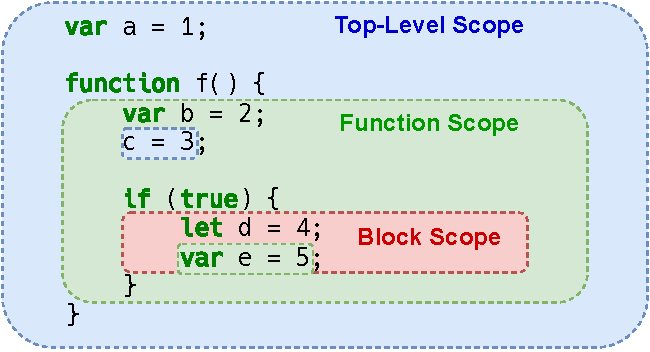
\includegraphics[width=9cm]{img/scope-4spaces.pdf}
    \caption{Scope of declared variables}
    \label{fig.scope}
\end{figure}

An example of variable declarations and the scope that they are bound to can be seen in \autoref{fig.scope}. Due to its definition in the top-level scope, the variable \icode{a} is bound to the global scope and visible to all scopes. In the function \icode{f}, the variable \icode{b} is bound to the function scope, while \icode{c} is part of the global scope, as it was not declared before the assignment. In the \icode{if} block, \icode{d} is part of the block scope due to the usage of \icode{let}, but \icode{e} is bound to the function scope, as \icode{var} does not bind variables to block scopes. Note that the function \icode{f} is also a global variable due to its definition in the top-level.



\subsection{Global Object}
\label{sec.globals}

The “global object” is an object that is always available in the global scope. Adding properties to the global object results in them also being accessible in the global scope. Global variables declared with \icode{var} and functions in the global scope are stored as properties of the global object, while variables created using \icode{let} and \icode{const} do not create such properties. The name of the global object varies depending on the context of where the code is executed. JavaScript code running in a web browser generally has a global object called \icode{window}, while web workers, which allow websites to execute JavaScript in the background and listen for notifications, use the global object \icode{WorkerGlobalScope} instead, and in Node.js the global object is simply called \icode{global}. \cite{MozGlobal}

The \icode{window} object represents the tab or window of the page running the code and provides an interface to various functions, including \hyperref[sec.browserAPIs]{browser APIs}. Its properties are generally isolated from other windows, with the exception of interfaces such as \icode{window.opener}, which are specifically designed to provide access to another window under certain conditions. \cite{MozWindow}



\subsection{Prototypes}
\label{sec.prototypes}

Similar to the typical class-based inheritance models of other object-oriented programming languages, JavaScript objects can inherit features from other objects via so-called prototypes. All JavaScript objects have a built-in property called prototype, which is an object itself and can also have a prototype, thereby creating a chain called the prototype chain. When accessing properties of an object, such as variables or methods, the property will first be looked for in the object itself. If the object does not contain a property, the prototype chain will be recursively traversed until either the desired property is found or \icode{null} – the end of the chain – is reached, in which case the resulting value will be \icode{undefined}. \cite{ECMA262_edition6, MozObjectPrototypes}



\subsection{Browser APIs}
\label{sec.browserAPIs}

Client-side web \acsp{api} are \acp{api} that are not built into the JavaScript language itself, but instead provided by the browser and its JavaScript engine. For the sake of clarity and readability this category of \acp{api} will be referred to as “browser \acsp{api}”.

Browser \acsp{api} consist of interfaces that allow scripts to interact with the page they are associated with, the browser, the device running the browser, device sensors and potentially also other connected devices. \acsp{api} not only expose additional features, but also act as an abstraction for the complexity associated with the implementation of commonly required functionalities to provide a simple interface for developers. \cite{MozWebAPIs}
One such interface is the \icode{document} object, which allows scripts to interact with the \ac{dom} and dynamically change the contents of \acs{html} documents through methods such as \icode{document.createElement()}, which creates a new element that can then be inserted into the page using methods such as \icode{document.body.append()} \cite{dom}. Another example is the fetch \acs{api}, which allows web applications to invoke network requests to dynamically send and receive data \cite{fetch}.

Furthermore, browser \acsp{api} also provide security related interfaces that handle sensitive data, such as the web authentication \acs{api} which allows web applications to implement secure authentication \cite{webauthn} or the web cryptography \acs{api} which provides secure implementations of common cryptographic algorithms that allow web applications to encrypt, decrypt, sign and verify data while abstracting the underlying implementations, secure key generation and management \cite{crypto}.

Browser APIs are globally accessible through the \hyperref[sec.globals]{global object} introduced in \autoref{sec.globals} and can generally be overwritten. The modification of browser \acsp{api} is not necessarily malicious, as it can be used to customize their behavior or, in the case of \hyperref[sec.polyfill]{polyfills}, to ensure the availability of certain \acsp{api} and provide consistent interfaces for web applications. This will be explained in more detail in \autoref{sec.polyfill}.



\section{Polyfills}
\label{sec.polyfill}

The term polyfill describes code that replicates the functionality of \acp{api} in environments that do not support them, such as outdated browsers. It usually refers to JavaScript code running in the browser that ensures the availability of certain \hyperref[sec.browserAPIs]{browser APIs} and that these \acsp{api} behave as defined by current or future specifications, regardless of the browser used to access the web application. In contrast to the term “shim”, polyfills provide a standardized interface for developers that acts as a “drop-in” replacement for the desired \acsp{api} instead of defining a new \acs{api}. \cite{MozPolyfill, RemyPolyfill}

Polyfills should only be used as a fallback, in case the required \acs{api} is not available or does not behave as expected, since their performance is not as good as that of native implementations and it is possible that they only support a subset of the full functionality. \cite{MozPolyfill}

As an example, we will take a look at how one would go about implementing a polyfill for the \icode{<String>.includes()} method, which can be called on strings to check if a string contains a given substring. This method was first specified in the 6th edition of ECMAScript published in 2015 \cite{ECMA262_edition6} and is therefore not implemented in old browsers such as Internet Explorer. Ideally, a polyfill should first check for the existence of a native implementation, which in this case can be achieved by evaluating \icode{String.prototype.includes}. If the function does exist in a browser, the aforementioned expression evaluates to true, meaning no polyfill is necessary. However, if it evaluates to false and thus does not exist, the code should add its own reimplementation of the includes function as a property of \icode{String.prototype}.

In the case of the \icode{<String>.includes()} method, a reimplementation of the native \acs{api} is trivial, as one can make use of the \icode{<String>.indexOf} method, which has been available since the first edition of ECMAScript published in 1997 \cite{ECMA262_edition1} and is therefore supported in all browsers. Aside from argument validation, the polyfill function only needs to call \icode{this.indexOf(search, start)}, which returns the position of a given substring in another string, and return \icode{true} if the position is $\ge 0$ and \icode{false} if the position is equal to $-1$, since the latter indicates that the string does not contain the given substring.



\section{Browser Extensions}
\label{sec.browserExtensions}

Browser extensions are a bundle of scripts and other resources that can add new functionality to a browser or change its behavior and \ac{ui} \cite{MozBrowserExtensions}. Browser extensions are generally written in JavaScript since all major browsers provide JavaScript \acsp{api} for extensions \cite{MozBrowserExtensionAPIs}. In addition to the \hyperref[sec.browserAPIs]{browser APIs} accessible to web pages, browser extensions have access to the browser extension \acsp{api}, which provide interfaces to control browser functionality such as bookmarks, tabs, notifications, browsing history, and are also able to intercept network requests and modify the content of web pages \cite{MozBrowserExtensions}.



\section{Origin and Same-Origin Policy}
\label{sec.origin}

Origins play an important role in the common security model used by browsers, known as the Same-Origin Policy. They are used to define which resources should be isolated from one another to prevent potentially malicious sites from accessing or interacting with third-party resources and reduce possible attack vectors. Pages of one origin usually only have limited or no access to resources that are part of a different origin. Data stored using the localStorage \acs{api} for example is only shared across the same origin, while cookies can also be shared across different origins \cite{html}. \cite{MozSameOriginPolicy}

The origin of a resource is determined by three parts of its \ac{uri}: scheme, domain and port. All resources with a matching triple of scheme, domain and port are part of the same origin. \cite{origin} The \acp{url} \icode{https://example.com/lorem} and \icode{https://example.com/ipsum} share the same origin, while \icode{http://example.com/lorem} and \icode{https://www.example.com/lorem} each have different origins, both from one another and from the first two \acp{url}, due to the difference in scheme and host respectively.



\section{Content Security Policy}
\label{sec.csp}

The \acf{csp} is a security feature that allows detecting and preventing the unintentional injection of resources into a web page by granularly declaring the sources where dynamic resources are allowed to be loaded from. It is intended to mitigate attacks such as \acf{xss} and monitor inclusions of untrusted resources in web applications. \cite{MozCSP}

To configure the policy, a web server needs to send the \icode{Content-Security-Policy} \acs{http} header with a valid policy configuration, or alternatively specify it using a \icode{<meta>} element in the \acs{html} document \cite{MozCSP}. For example, the following policy shown in listing \ref{lst.csp} could be used in order to block resources from everywhere except for the sites own origin, but allow images and other media to be loaded from the domain \icode{cdn.example.com}.

\begin{lstlisting}[language=CSP,numbers=none,label={lst.csp},caption={Example of a valid CSP policy}]
default-src 'self'; img-src cdn.example.com; media-src cdn.example.com
\end{lstlisting}

It is also possible to configure the \ac{csp} such that browsers send reports about violations of the policy to a desired endpoint using the \icode{report-uri} directive. The endpoint will receive reports in the form of \acs{json} encoded data. \cite{MozCSP}



\section{Browser Security Architecture}
\label{sec.browser-security-architecture}

This section explains the core concepts of the security architectures of browsers. It primarily focuses on the security architectures of Chromium and Firefox, which share similar approaches, but the concepts discussed here are also applicable to other browsers. Both Chromium and Firefox isolate the processing and rendering of web content from the rest of the browser and its \ac{ui}. Every web page has a separate rendering process, which is responsible for functionality such as parsing \acs{html}/\acs{css}, decoding images, interpreting JavaScript code, handling the \ac{dom} and rendering the page. Due to the complexity of the rendering engine and the fact that it needs to handle untrusted data from the web, these processes run in a sandbox that prevents them from directly accessing certain functionality of the \ac{os}. The sandbox is configured to have as few permissions as possible and prevents access to the filesystem – with a few exceptions such as temporary files that depend on the browser and \ac{os} – and also prevent access to the network. In order to send and receive data to/from the network, the rendering processes communicate with the main browser process using \ac{ipc}.~\cite{ChromiumSecArchitecture, MozFFSandbox}

\begin{figure}[H]
    \centering
    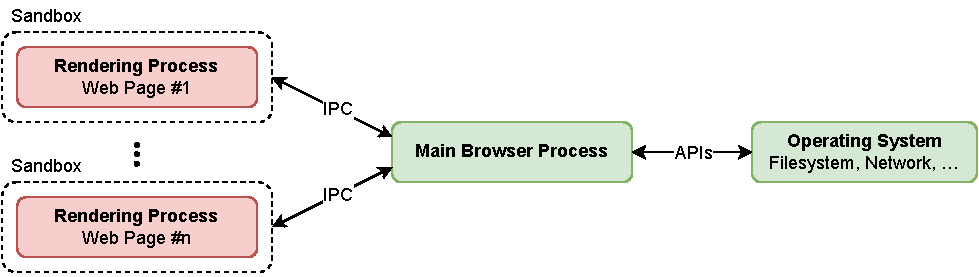
\includegraphics[width=16cm]{img/browser-process-model.pdf}
    \caption{Simplified Browser Process Model}
    \label{fig.browser-process-model}
\end{figure}

\autoref{fig.browser-process-model} depicts a simplified version of the actual process model, which also contains separate proccesses for \acs{gpu} rendering, browser extensions and more. The colors of the boxes represent the “trustworthyness”, with the red rendering process being considered untrusted due to its execution of potentially malicious code, while the green main browser process and \ac{os} are considered to be trusted. The sandbox allows the different trust environments to be isolated from each other and only interact through limited interfaces over \acs{ipc}. This means that even in a case where malicious web content manages to execute arbitrary code inside the rendering process through a security vulnerability, it would still not be able to access the filesystem, due to the restrictions of the sandbox. \cite{ChromiumSecArchitecture, MozFFSandbox}



% ============================ Related Work ============================
\chapter{Related Work}
\label{sec.relatedwork}

This chapter summarizes related work that investigates the inclusion of externally hosted JavaScript code, the security implications, and mitigation attempts. Furthermore, it presents security research related to JavaScript vulnerabilities. The former topics will be relevant for the threat model of this thesis.

\citeauthor{JSinclusions}~\cite{JSinclusions} conducted a large-scale evaluation of remote JavaScript inclusions in the most popular \num[round-precision=0]{10000} domains of the Alexa ranking over a period of ten years. As part of the evaluation, the researchers downloaded yearly snapshots of web pages hosted on these domains and processed more than three million pages in total. They analyzed the trust relationships between the sites and the providers of the remote scripts that they include and also assessed the maintenance quality of those providers based on metrics such as the security rating of the \acs{ssl}/\acs{tls} configuration and whether the server software was up-to-date.

The results of the evaluation of \citeauthor{JSinclusions} show that it is common practice for sites to include remote code, with \SI[round-precision=2]{88.45}{\percent} of the domains including at least one JavaScript library form a third party. Even though the majority of domains only include code from a few remote hosts, a small amount of popular sites include JavaScript libraries from up to \num[round-precision=0]{295} different remote hosts. It was also discovered that the amount of remote inclusions is steadily growing, reaching an average of \SI[round-precision=2]{2.10}{\percent} new unique domains per year in 2010. The study came to the conclusion that the inclusion of remote JavaScript libraries increases the attack surface and poses a threat to the security of web applications. When developers include remote JavaScript code in their web applications, they implicitly trust the providers of this code, since the latter have complete control over it and could execute malicious code at any time. This would give attackers the ability to steal user credentials or deface the site. The analysis regarding the quality of maintenace of the providers identified that a considerable amount of popular websites include code from third-parties that did not meet the best practices and security-standards imposed by the authors, which could lead them to be compromised by attackers. \cite{JSinclusions}

Another study \cite{ThirdPartyResources} analyzed the dependency chains created by third-party resources that include additional third-party resources themselves. Web applications that have these dependency chains place implicit trust on transitively included resources, which further increases the attack surface. Out of the \num[round-precision=0]{200000} most popular websites that were analyzed, \SI[round-precision=0]{91}{\percent} included JavaScript code from external hosts and around half of the websites implicitly include resources through a chain of dependencies. While \SI[round-precision=2]{84.91}{\percent} of the dependency chains do not exceed a length of three levels, the longest dependency chain reached a total length of \num[round-precision=0]{38} levels. The authors argue that complex chains of transitive inclusions make it difficult to reliably audit web applications, since is not possible to guarantee which resources will be included later on. The study also analyzed the third paries using VirusTotal and classified \SI[round-precision=2]{1.20}{\percent} of them as suspicious. The majority~(\SI[round-precision=0]{73}{\percent}) of websites that include resources from suspicious third-parties included them explicitly, which leads the authors to the conclusion that website operators are not thoroughly monitoring their external dependencies.

\citeauthor*{InBrowserDetection} \cite{InBrowserDetection} noted that, with increasing frequency, third-party content such as advertisements is also being injected by \acp{isp} and browser extensions for monetary benefits. Meanwhile, attackers use these advertisements to distribute malicious code. To defend against these types of injections, the authors developed an approach called “Excision”, which consists of modifications to the source code of the Chromium browser that analyzes the sequence of inclusions in order to identify and block malicious third-party content. Unlike traditional approaches, this method does not analyze the content of third-party resources, only the chain of inclusions that lead to the inclusion of the content in question. This method allows to combat common obfuscation techniques that attackers use to evade detection. To verify the effectiveness of their approach, an evaluation was performed, in which the modified browser analyzed the domains of the Alexa Top 200K ranking list over a period of eleven months. The results of the evaluation show that it has a high detection rate of \SI[round-precision=2]{93.39}{\percent} while maintaining a low false positive rate of \SI[round-precision=2]{0.59}{\percent}. An evaluation of the impact on performance showed that users did not notice a significant impact on their browsing experience.

To defend against the inclusion of malicious third-party content, \citeauthor*{InBrowserDetection} recommended the use of in-browser detection algorithms such as Excision in addition to techniques such as the \ac{csp}. They noted, however, that the \ac{csp} can be defeated by \acp{isp} and browser extensions since both of these parties are able to modify or remove the headers that are used to define this policy.

Additionally, there is research that focuses on JavaScript vulnerabilities. In \cite{Steffens_2021} Steffens discusses various client-side vulnerabilities, including Prototype Pollution. The thesis identified the presence of investigated vulnerabilities even among the most popular sites and concluded that there is a need for automated tools to assist web developers in detecting vulnerabilities. \cite{Steffens_2021}



% =============================== Threats ==============================
\chapter{Threats of Browser API Manipulation}
\label{sec.threats}

This chapter investigates the implications of \browserAPI{} manipulation and, through several examples, demonstrates the threats that this can pose. The term “\browserAPI{} manipulation” refers to the modification or overwriting of JavaScript \acsp{api} provided by the browser engine. While manipulation of \acsp{api} is not inherently malicious, as explained in the fundamentals \autoref{sec.browserAPIs} and \autoref{sec.polyfill} about Browser APIs and Polyfills, this chapter only addresses the malicious use-cases. First, \autoref{sec.threatmodel} presents the threat model that this investigation is based on. Then, the following sections describe potential threats, with each section focusing on a specific group of \acsp{api} that share similar properties and implications. An overview of these threats can be seen in \autoref{tab.threats}.

\begin{table}[h]
    \parbox{\linewidth}{
    \centering
    \begin{tabularx}{\textwidth}{l|p{30mm}|p{45mm}|X}
        Section & Affected APIs & Threats & Implications \\
        \hline
        \ref{sec.threats.requestinterception} &
        \minline{fetch}, \minline{XMLHttpRequest} &
        Interception and manipulation of network requests that originate from scripts &
        Compromises data integrity by allowing manipulation of data being sent and received;
        Can be used for application layer \acs{ddos}~attacks
        \\\hline
        \ref{sec.threats.crypto.plaintext} &
        \minline{crypto.subtle} &
        Access to plain-text data before it is encrypted &
        Compromises data confidentiality by allowing access to and exfiltration of unencrypted data
        \\\hline
        \ref{sec.threats.entropy} &
        \minline{crypto} &
        Manipulation of pseudo random numbers &
        Compromises security of passwords, tokens and cryptographic keys generated based on random numbers
        \\\hline
        \ref{sec.threats.intercept-privileged} &
        privileged APIs such as Geolocation or Web Authentication &
        Intercept requests to sensitive data and credentials &
        Compromises the confidentiality of sensitive data; Stolen credentials can be used for impersonation
    \end{tabularx}
    \caption{Summary of threats presented in this chapter}
    \label{tab.threats}
    }
\end{table}



\section{Threat Model}
\label{sec.threatmodel}

This section presents the threat model that the investigation of threats is based on. Contrary to conventional threat models (cf. \cite{ChromiumSecArchitecture}), which generally have the goal of developing countermeasures against threats, this threat model assumes that web applications are vulnerable in order to assess the resulting threats. The primary goal of this thesis is to \textit{detect} the threats, which will be discussed in \autoref{sec.detection}. In the first part of this section, we will take a look at the roles and components of the threat model and visualize how they interact with each other. Then, potential entry points for code execution are presented and finally, the attackers' goals are defined, as well as their abilities and limitations.

The considered threat model includes the following main components: the user, browser, browser extensions, web servers and web application code. \autoref{fig.threat-model-components} shows the relationship and interactions between these components. The user interacts with the browser, e.g. visits a website and interacts with dialogs. The browser communicates with web servers over the internet, which are responsible for relaying the web application code. Web applications consist of first party code and can also include code from third-parties. This can either be done directly, when the third-party code is hosted on the first party web server, or by indirectly including the code from third-party servers such as a \ac{cdn}. Third-party servers can also be used to deliver first party code.

\begin{figure}[H]
    \centering
    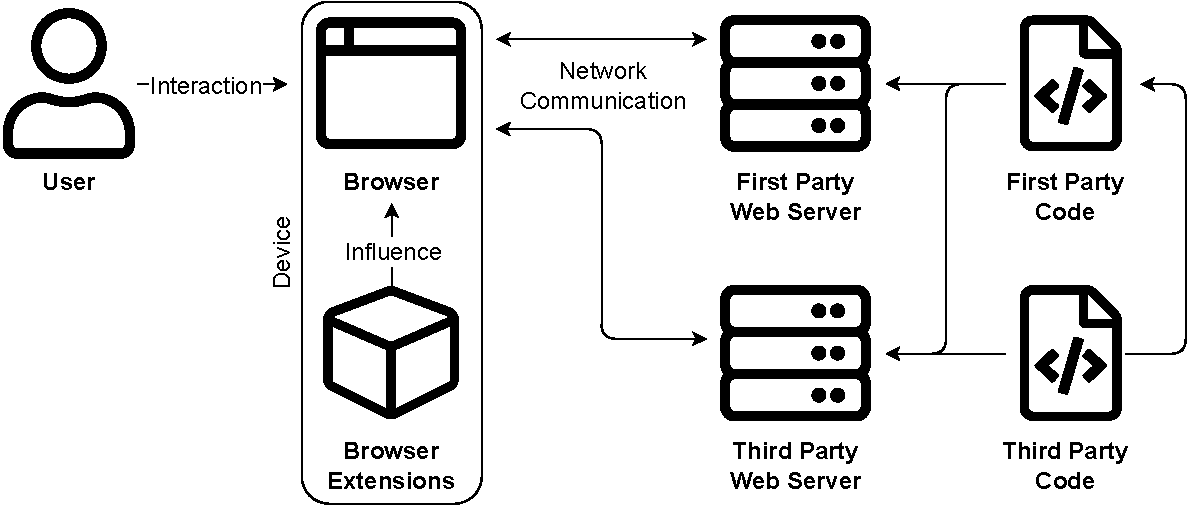
\includegraphics[width=13.9cm]{img/threat-model.pdf}
    \caption{Components of the Threat Model}
    \label{fig.threat-model-components}
\end{figure}

\BrowserAPIs{} are accessible through the \hyperref[sec.globals]{global \icode{window} object} and can be overwritten the same way as any other variable (cf. \autoref{sec.browserAPIs}). As the window object is not shared across different web pages, an attacker needs to be able to execute JavaScript code in the context of the targeted web page in order to manipulate \browserAPIs{}. This can be achieved in the following cases:

\begin{enumerate}
    \item If security vulnerabilities are present in a web application that allow an attacker to execute code in the users browser, such as \ac{xss} vulnerabilities.
    \item Through \ac{mitm} attacks that intercept the communication between the browser and web servers, allowing the injection of arbitrary code. This is possible when the connection is insecure, e.g. when \acs{http} is used instead of \acs{https}.
    \item If the attacker is able to modify third-party code that is included in the web application. This could, for example, be an open-source library that the attacker has control over.
    \item When the attacker is able to control a third-party web server that hosts code included in the web application.
    \item If the browser is running an extension that is controlled by the attacker and has the required privileges to inject code into web pages.
\end{enumerate}

The attacker can visit websites and analyze them for security vulnerabilities and JavaScript inclusions. The analysis may reveal possible points of entry as listed above. If an attacker detects the usage of third-party JavaScript code in a web application, they can attempt to modify the official distribution source, either where the code is downloaded from or where it is remotely included from. If the third-party JavaScript code originates from an open-source project, the attacker could attempt to contribute malicious code to it, in order for it to eventually be distributed. The attacker can also analyze the dependency chains of remote inclusions as well as the dependency chains of libraries that the web application uses. This can reveal additional entry points that can be compromised.

The execution of JavaScript code allows an attacker to control a web application and access associated data such as cookies and the local storage. Here, we will only focus on the threats posed by \browserAPI{} manipulation and not the usage of \browserAPIs{}.

There are, however, some restrictions to the constructed attacker. The attacker is not able to access data from other web applications. Due to the browser security architecture described in \autoref{sec.browser-security-architecture} and the same origin policy explained in \autoref{sec.origin}, it is generally not possible for an attacker to access data of other web pages. The browser security architecture also makes it impossible for the web application to access the filesystem unless users explicitly choose and grant access to a file themselves.

The attacker considered in this threat model has at least one of the following goals:

\begin{enumerate}
    \item Impersonate users through a web application. This includes performing actions as the targeted user inside of the web application and signing or encrypting data as the user.
    \item Manipulate the behavior of web applications and the users actions. This can, for example, include modifying the information that is sent and displayed to the user or modifying the data that the user sends to the web application.
    \item Access private data from users that is controlled by the web application. This includes cryptographic keys and plaintext before it is encrypted.
    \item Cause a denial of service of the web application.
\end{enumerate}



\section{Network Request Interception and Manipulation}
\label{sec.threats.requestinterception}

\minline{Fetch} and \minline{XMLHttpRequest} are \browserAPIs{} that allow sending \acs{http} requests. Overwriting them would give an attacker control over the data being sent and received by a web application. This is effectively a \ac{mitm} attack limited to network requests originating from JavaScript code and allows an attacker to intercept and manipulate users actions and data, thereby compromising data integrity. This also allows attackers to cause a client-side \ac{dos} which can be used to target specific users and prevent them from using the web application or even specific functionality of the application.

Furthermore, attackers can use these \acsp{api} for an application layer \ac{ddos}~attack by amplifying the amount of requests generated by users. Unlike traditional \ac{ddos}~attacks, which target the network layer using techniques such as \acs{udp} or \acs{tcp}~SNY flooding, application layer \ac{ddos}~attacks are designed to flood the web application with legitimate requests that are computationally expensive to process. For attackers, this has the benefit of being more effective at overloading the targeted systems and harder to mitigate due to requests being indistinguishable from ones generated by legitimate users. \cite{ApplicationLayerDDoS}

As an example of request manipulation, let us take a look at a hypothetical banking web application that allows transferring money to a recipient, which is implemented by sending transaction data encoded as \acs{json} to a \acs{rest}~\acs{api} reachable at \minline{/api/transfer-money}. To send the data, the web application uses the \minline{fetch}~\acs{api}, as shown in listing \ref{lst.fetchExample}. If an attacker were to inject code that changes the behavior of \minline{fetch}, such that it would examine and change data before being sent, it would be possible to change the behavior of the web application without needing to change the specific code of the application that is responsible for processing user input and sending the data.

\begin{lstlisting}[language=JavaScript,label={lst.fetchExample},caption={Fetch request with \acs{json} data}]
fetch("/api/transfer-money", {
    method: "POST",
    body: JSON.stringify({
        recipient: "Alice"
    })
});
\end{lstlisting}

Listing \ref{lst.fetchManipulation} shows code that, when injected, stores a reference to the original \minline{fetch}~\acs{api} and then overwrites \minline{fetch} with code that replaces the recipient in the \acs{json} data passed to it with \minline{"Eve"} and then sends the modified request using the original \minline{fetch}~\acs{api}. This would result in all transactions now being sent to Eve, instead of Alice.

\begin{lstlisting}[language=JavaScript,label={lst.fetchManipulation},caption={Overwriting fetch to manipulate data under certain conditions}]
// Store original fetch
const originalFetch = window.fetch;

// Overwrite fetch
window.fetch = (resource, init) => {
    // Only change request under certain conditions
    if (resource === "/api/transfer-money") {
        if (typeof init?.body === "string") {
            let data = JSON.parse(init.body)
            data.recipient = "Eve";
            init.body = JSON.stringify(data);
        }
    }
    // Send request via original fetch API
    return originalFetch(resource, init);
};
\end{lstlisting}



\section{Cryptography Backdoors}
\label{sec.threats.crypto}

The Web Cryptography \acs{api} provides an interface for web applications to generate and store cryptographic keys, which can be used to encrypt, decrypt, sign and verify data. The interfaces can be accessed through the globally accessible \icode{crypto} and \icode{crypto.subtle} objects. While the objects themselves are defined to be read-only, their methods can be modified, which allows changing their behavior. \cite{crypto}

Most of these \acs{api} methods, with the exception of \icode{crypto.getRandomValues()}, are only available in a secure context, such as pages loaded over \acs{https} \cite{crypto}. This prevents the use of functions intended to handle sensitive data in an insecure context, as this could otherwise make it possible for attackers to inject code or manipulate data using a \ac{mitm} attack.



\subsection{Data Exfiltration}
\label{sec.threats.crypto.plaintext}

An attacker could modify the \icode{crypto.subtle.encrypt} method such that data is exfiltrated before it is encrypted. An example of this is shown in \autoref{lst.encrypt-middleware}, where first, a reference to the original method is stored and then the method is overwritten to decode and log the plaintext. Finally, the arguments are passed along to the original method and its result is returned. Instead of logging the text, it could also be exfiltrated using the fetch \acs{api} to send the data to a webserver controlled by the attacker. It would also be possible to first store the data locally and exfiltrate it at a later time to obfuscate the malicious behavior and reduce the chance of detection.

\begin{lstlisting}[language=JavaScript,label={lst.encrypt-middleware},caption={Interception of data before it is encrypted}]
// store reference to original function
let origEncrypt = crypto.subtle.encrypt;

// overwrite the API
crypto.subtle.encrypt = (algorithm, key, data) => {
    // access the plaintext before it is encrypted
    let decoder = new TextDecoder();
    let plaintext = decoder.decode(data);
    console.log("Plaintext:", plaintext);

    // call the original function and return the encrypted data
    return origEncrypt.apply(crypto.subtle, [algorithm, key, data]);
};
\end{lstlisting}



\subsection{Entropy Manipulation}
\label{sec.threats.entropy}

Another method of the Web Cryptography \acs{api} is \icode{crypto.getRandomValues()}, which takes a typed array as an argument, e.g. a \icode{Uint8Array} or \icode{Int32Array}, and overwrites all elements of the provided array with cryptographically strong random values matching its type \cite{crypto}. The specification states that implementations should seed the \ac{prng} with a good source of entropy, such as the source provided by the \ac{os}, but does not contain any requirements to the level of entropy guaranteed by the \acs{api}. While this method should not be used to generate cryptographic keys, it can be used to generate random tokens, passwords or any other sequence that is required to be random.

It is possible to overwrite \icode{getRandomValues()} and thereby compromise the integrity of any code that depends on the entropy of its result. An attacker could replace the method with a function that returns a known sequence instead of a random one, as shown in \autoref{lst.random-fixed-value} where the provided array is filled with the fixed value \icode{4}.

\begin{lstlisting}[language=JavaScript,escapeinside={/*!}{!*/},escapebegin=\itshape\color{magenta!90!black},label={lst.random-fixed-value},caption={Returning fixed instead of random values.}]
crypto.getRandomValues = array => {
    array.fill(4); // /*!\href{https://xkcd.com/221/}{chosen by fair dice roll.}!*/
                   // /*!\href{https://xkcd.com/221/}{guaranteed to be random.}!*/
    return array;
};
\end{lstlisting}
% https://xkcd.com/221/
% https://dilbert.com/strip/2001-10-25

A more sophisticated attack could provide a polyfill that generates seemingly random values while actually choosing values that follow a pattern known to the attacker. This could also be achieved using a \ac{prng} with a known seed or a predictable seed with a low quality of entropy.



\section{Intercepting Privileged APIs}
\label{sec.threats.intercept-privileged}

\BrowserAPIs{} that allow web applications to request access to sensitive information, such as Geolocation, require users to give their consent by confirming a dialog that prompts them for permission. In order for an attacker to use these \acsp{api}, they would need to get users to confirm such a dialog. This requires attackers to convince users of two things: first, that the website needs the data that is being requested and second, that the website is trustworthy. Traditional approaches such as phishing might not be able to convince users of these statements. If an attacker is able to overwrite these \browserAPIs{} on a web application that the user already trusts, they can simply wait for the web application to request the permission to access the sensitive information and intercept the response once access has been granted. The response can be intercepted by storing a reference to the \ac{api} function and overwriting the browser \ac{api} with a new function that acts as an intermediary by calling the reference of the original \ac{api} and exfiltrating the response data.

Another \ac{api} that is relevant to the goals of the attacker is the Web Authentication \ac{api}, which is used to securely authenticate a user through a web application \cite{webauthn}. One of the security features of the \ac{api} is that it prevents phishing sites from stealing credentials by binding the credentials to the origin of a site \cite{webauthn}. Intercepting calls from a web application to this \ac{api} would allow attackers to steal the credentials associated with the site and use them to gain access to the users account and impersonate them.



% ============================== Detection =============================
\chapter{Detection of Browser API Manipulation}
\label{sec.detection}

This chapter deals with the implementation of algorithms that can detect \browserAPI{} manipulation. These algorithms will be relevant for \autoref{sec.browserExtension}, where a browser extension is implemented that automatically analyzes web pages using these algorithms and presents their results to the user. The following sections describe possible approaches on how to implement these detection algorithms and compares their benefits and drawbacks. The first approach presented in \autoref{sec.detectionInterception} attempts to intercept code that overwrites \browserAPIs{}, while the second approach in \autoref{sec.detectionVerification} detects changes to \browserAPIs{} by continuosly verifying their integrity. The latter achieves this through two methods: The first method stores references of the original values and verifies whether the current state matches the references, and the second one scans \browserAPIs{} for built-in functions that have been replaced by a non built-in function.



\section{Interception of Browser API Overrides}
\label{sec.detectionInterception}

The first approach to detect \browserAPI{} manipulation is to intercept code that wants to overwrite existing \acp{api}. While this could be done at different stages of the code execution pipeline, it is difficult to impossible to detect whether a script will overwrite certain properties at some point just from static analysis of the code. Static code analysis could easily be fooled by code obfuscation and would require complex syntactical parsing and code flow analysis. Instead, the approach presented here effectively performs a dynamic code analysis by making use of JavaScript's setter functions in order to intercept attempts at overwriting certain properties of the \hyperref[sec.globals]{global object} introduced in \autoref{sec.globals}.

It is possible to add setter functions to properties of JavaScript objects using the method \icode{Object.defineProperty()}. Adding a setter function, however, prevents one from storing a value inside of the property. To make sure that the property still has the same value that it had before defining a setter function, we also need store the original value in another variable (referred to as the “shadow variable“ – not to be confused with “variable shadowing”), define a getter function that returns the value of the shadow variable and assign values received by the setter function to the same shadow variable. \cite{MozObjectDefineProperty}

\autoref{lst.observeOverwrites} shows a function that implements the aforementioned steps and allows adding a hook function to an object's setter which will be called whenever a value is written to the specified property of the parent object. In line 9, a shadow variable is created, which keeps track of the value associated with the property. The function can then be used to observe specific \acp{api}, such as \icode{fetch}, by calling it as shown in listing \ref{lst.observeFetchOverwrite}. In this case, the hook function simply logs a warning message whenever a new value is assigned to fetch, including a stack trace of the code that was responsible for the value change.

\filbreak{}

\begin{lstlisting}[language=JavaScript,label={lst.observeOverwrites},caption={Function that can be used to observe overwrites of an object's property}]
/**
 * Observes overwrites of a property.
 * @param {Object} obj Parent object
 * @param {String} prop Property name
 * @param {Function} hook Hook function.
 */
function observeProperty(obj, prop, hook) {
    // Store original value in shadow variable
    let shadow = obj[prop];
    Object.defineProperty(obj, prop, {
        // Define setter
        set: value => {
            // Call hook function
            hook();
            // Store value in shadow variable
            shadow = value;
        },
        // Define getter to return value of shadow variable
        get: () => shadow,
    });
};
\end{lstlisting}

\begin{lstlisting}[language=JavaScript,label={lst.observeFetchOverwrite},caption={Observing changes to the fetch API}]
observeProperty(window, "fetch", () => {
    console.warn("fetch was overwritten. Stack Trace:", (new Error()).stack);
});
\end{lstlisting}

The approach demonstrated in this subsection has the benefit that changes are detected immediately and it is also possible to trace the callstack in order to find out what part of the code was responsible for overwriting an \ac{api}, which will be relevant for the implementation of the browser extension in \autoref{sec.browserExtension}.

On the downside, this not only requires the definition of setter functions for every single property, but also copying all of the original values to shadow variables. It is also possible to circumvent the detection by using \icode{Object.defineProperty()} or \icode{Object.defineProperties()} to either remove the setters or overwrite the value directly.

To improve the detection rate, one could additionally attach a hook to the aforementioned methods to intercept their use. This could be done using a helper function as shown in listing \ref{lst.hookFunction}, which simply replaces the specified property with another function that first calls the provided hook function, then calls the original function and returns its result. This helper function is then used in listing \ref{lst.hookDefineProperty}, which uses the helper function from listing \ref{lst.hookFunction} to attach hooks to \icode{Object.defineProperty()} and \icode{Object.defineProperties()} that log a warning with a stack trace whenever the methods are used to overwrite properties of the global \icode{window} object.

\filbreak{}

\begin{lstlisting}[language=JavaScript,label={lst.hookFunction},caption={Function that allows adding a hook to another function}]
/**
 * Adds a hook to a function.
 * @param {Object} obj Parent object
 * @param {String} prop Property name
 * @param {Function} hook Hook function.
 */
function hookFunction(obj, prop, hook) {
    // Store a reference to the original function
    let originalFunction = obj[prop];
    // Replace function
    obj[prop] = (...args) => {
        // Call hook
        hook(...args);
        // Call original function and return the result
        return originalFunction(...args);
    }
}
\end{lstlisting}

\begin{lstlisting}[language=JavaScript,label={lst.hookDefineProperty},caption={Adding hooks to \icode{Object.defineProperty()} and \icode{Object.defineProperties()}}]
hookFunction(Object, 'defineProperty', (obj, prop, descriptor) => {
    if (obj !== window) return;
    console.warn(prop+" was overwritten. Stack Trace:", (new Error()).stack);
});
hookFunction(Object, 'defineProperties', (obj, props) => {
    if (obj !== window) return;
    console.warn("Multiple properties overwritten:", Object.keys(props), "Stack Trace:", (new Error()).stack);
});
\end{lstlisting}

\section{Integrity Verification of Browser APIs}
\label{sec.detectionVerification}

The second approach to detecting \browserAPI{} manipulation is to verify the integrity of the associated JavaScript objects and functions instead of intercepting code. A possible solution for achieving this would be to store references of the initial state and then continuously compare them to the current values. The downside of this approach is the computational and memory overhead required to copy, store and compare the references and that – compared to the first approach – this does not immediately detect manipulation, but instead requires actively scanning the \acp{api} for changes to their values.

Functions provided by the browser can alternatively also be verified by checking their string representation. The \icode{toString()} method of the \minline{Function.prototype} returns the string representation of a function \cite{ECMA262}, which generally matches the source code of the function object. However, in the case of built-in function objects this function returns an implementation-defined string \cite{ECMA262}, which can be used to verify that a function is built-in and thus not modified.

As the specification only defines the syntax of the string representation of built-in function objects, the exact representation is only guaranteed to be consistent within a browser. The following code shown in \autoref{lst.builtinFuncString} can be used to generate the expected string representation independently of the browser it is running in.

\begin{lstlisting}[language=JavaScript,showstringspaces=true,label={lst.builtinFuncString},caption={Generating the expected string representation of built-in function objects}]
// Store a trusted reference to Function.prototype.toString
const funcToString = Function.prototype.toString;

/**
 * Returns the expected string representation of built-in functions.
 * @param {String} name Name of the function.
 * @returns {String}
 */
function builtinFuncString(name) {
    // Browser independent:
    return funcToString.apply(funcToString).replace("toString", name);
    // Chromium:
    return `function ${name}() { [native code] }`;
    // Firefox:
    return `function ${name}() {\n    [native code]\n}`;
}
\end{lstlisting}

However, this method of verification requires handling some special cases where the internal function name is different from the name of the \icode{window} object property that it is assigned to. This can occur on properties that are aliases of an \ac{api}, such as \icode{WebKitCSSMatrix} for example, which is an alias of \icode{DOMMatrix}. As these aliases behave like pointers, the internal name of the function does not reflect the property name of an alias. Chromium also provides \acp{api} that do not have an internal name in their string representation, such as \minline{chrome.loadTimes}.



% ============================== Extension =============================
\chapter{Implementation as a Browser Extension}
\label{sec.browserExtension}

As part of this thesis, a browser extension was developed that implements the detection methods presented in \autoref{sec.detection} and uses them to automatically analyze web pages that a user navigates to for any changes to \browserAPIs{}. As each of these approaches come with their own benefits and drawbacks, a combination of both of them will be used to improve the detection rate. The user is then informed about the result in the \ac{ui} through an icon that changes its color corresponding to the result (green, yellow, red). Additionally, clicking on this icon reveals a popup with a list of the affected APIs. While the extension can automatically detect \browserAPI{} manipulation and is simple to install and use, it is not able to classify whether the detected manipulation is legitimate or malicious, such as in the case of polyfills. This means that the extension is primarily aimed at web developers and security researchers that want to investigate the behavior of web applications and ensure that \browserAPIs{} are only overwritten when expected. The interpretation of a positive result – when manipulation was detected – unfortunately requires technical knowledge about the web application in question in order to know whether the manipulation is actually malicious or legitimate.

Even though in this case the detection tool was implemented in the form of a browser extension, the detection should ideally be builtin to the browser itself, as this would produce the most accurate results due to direct access to the internal memory state of the JavaScript context while also being isolated from it. However, not only is modifying and compiling a browser a considerably larger challenge than developing a browser extension, it also either requires the patch to be merged into the original (so-called “upstream”) code-base or constant maintenance to keep these patches compatible with the upstream. It is unlikely that such a patch would be merged into browsers and the alternative of patching and compiling a browser is not a viable solution to distribute the application for end users due to the required know-how and long compile times.

The first section \ref{sec.browserExtensionArchitecture} of this chapter will give an overview over the browser extension architecture and how its functionality was implemented. The second section \ref{sec.browserExtensionPolyfillDetection} will explain how the extension detects the use of polyfill libraries.

\filbreak{}

\section{Browser Extension Architecture}
\label{sec.browserExtensionArchitecture}

This section presents the architecture of the browser extension. An overview of the components and their interactions can be seen in \autoref{fig.browser-extension-context}.

\begin{figure}[H]
    \centering
    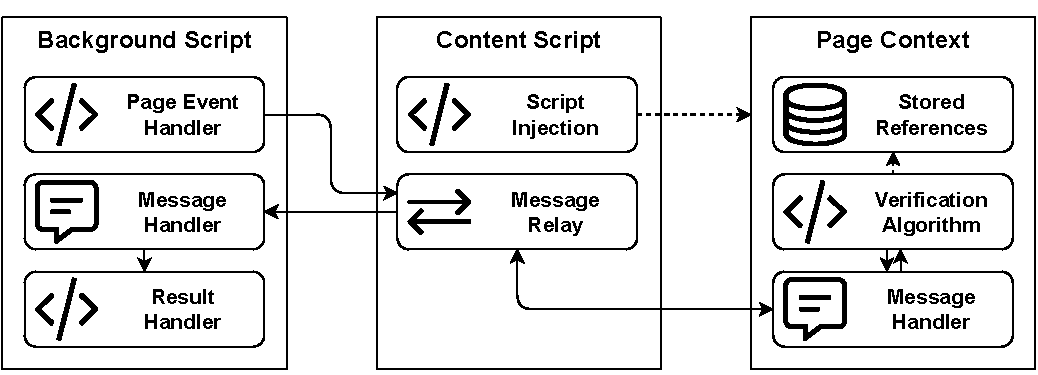
\includegraphics[width=16cm]{img/context-diagram.pdf}
    \caption{Browser extension architecture}
    \label{fig.browser-extension-context}
\end{figure}

The browser extension is responsible for injecting JavaScript code that makes use of the aforementioned detection mechanisms and displaying the results to the user. It is crucial that the code is injected and executed before any other code can be executed, including JavaScript code embedded in the original \acs{html} document itself.

Extensions are able to provide so-called “content scripts” which can access the \ac{dom}, but are sandboxed from the JavaScript context of the page and therefore also don't have access to the same \minline{window} object. In order to run code in the same context as the code of the page itself, a workaround is required: The content script creates a \minline{script} element and injects it into the \ac{dom} by prepending it to the \minline{head} or, as a fallback, the root \minline{document} element.
The desired code can either be provided by pointing the \minline{src} property to a script provided by the extension (which would need to be defined as a “web accessible resource“), or alternatively set the \minline{textContent} property to the string representation of the code. The latter allows dynamically creating the injected script, where one can make use of the fact that \minline{Function.prototype.toString()} returns the string representation of a function and \minline{JSON.stringify()} could be used to encode arguments passed to the function.

% \begin{lstlisting}[language=JavaScript,caption={Injecting JavaScript code into a page from a content script}]
% // Create new script element.
% const script = document.createElement("script");

% // Either provide a URL to the script
% script.src = browser.runtime.getURL("the-injected-script.js");
% // or provide the code as a string.
% const injectedFunction = () => {
%     // This will be executed in the page context.
%     window.foo = "bar";
% };
% const scriptAsString = "(" + injectedFunction.toString() + ")();";
% script.textContent = scriptAsString;

% // Prepend script to head, fallback to document root node.
% (document.head || document.documentElement).prepend(script);

% // Optionally, remove script after it was executed.
% script.remove();
% \end{lstlisting}

Another hurdle that gets in the way of script injection is the \hyperref[sec.csp]{\ac{csp} described in the fundamentals \autoref{sec.csp}}, which can be configured to deny execution of JavaScript code embedded into the \acs{html} document. While Chromium ignores the \ac{csp} for resources injected by extensions using the manifest v2 \acs{api}, this is no longer the case for extensions using manifest v3. Chromium manifest v3 extensions can instead directly execute code in the page context using \minline{chrome.scripting.executeScript()} with the \minline{ExecutionWorld} set to \minline{main}. However, this method can not be used here, since the provided code is no longer guaranteed to be executed first, which would allow JavaScript code to change properties before references are stored.

Firefox, unlike Chromium, treats resources injected by extensions the same way as page resources. This means that the extension only works when a page does not block inline scripts. A possible solution to this problem would be to use the Firefox-only Xray Vision \acs{api}, which allows direct access to a pages window object \cite{XrayVisionDocs}.

The next challenge is handling communication between the code running in the page context and the content script, in order for the extension to be able to request a verification and also get a result back. This can be solved by using \icode{window.postMessage()}, which allows posting a message that can contain any serializable Object to a given window. In both contexts a \icode{message} event listener is registered that checks received messages for a match and then acts accordingly.

Finally, the content script needs to relay messages between the page and the background script, which sends out the verification request after a page has finished loading and receives the response in order to display the results to the user. This communication happens in a similar manner, using the \icode{postMessage()} function of a \icode{runtime.Port} that connects both of the contexts.

The result is directly indicated to the user by the browser extension's action icon color. The icon is green when no changes to browser \acsp{api} are detected, yellow when there is no result, and red means that at least one change to a browser \acs{api} or other native function was detected.



\section{Polyfill Library Detection}
\label{sec.browserExtensionPolyfillDetection}

The browser extension detects polyfill libraries in two ways: scanning for the presence of global variable names that are used by polyfill libraries and by intercepting script inclusions if the \acs{url} matches patterns of known polyfill services.

It is possible to detect the polyfill library core-js due to a global variable that it creates. The library uses the global variable \icode{__core-js_shared__} to store information such as the version and certain function implementations in case different versions of the same library are used. As shown in \autoref{lst.detectcorejs}, the code for its detection only needs to check if the aforementioned variable name is a property of the global window object using the \icode{hasOwnProperty()} method.

\begin{lstlisting}[language=JavaScript,label={lst.detectcorejs},caption={Detection of the core-js library}]
if (Object.prototype.hasOwnProperty.call(window, "__core-js_shared__")) {
    // core-js detected
}
\end{lstlisting}

Some of the externally included polyfill libraries can be detected by filtering the scripts that a page includes and looking for \acsp{url} that match patterns of known polyfill services and library names. \autoref{lst.requestfilter} demonstrates how extensions can intercept requests using the \icode{webRequest.onCompleted} event. In order to limit events to scripts included by a page and requests originating fom JavaScript code, the type needs to be filtered to \icode{script} and \icode{xmlhttprequest}. The former type is assigned to requests for resources included using script elements, and the latter covers requests from scripts, which could in theory also be used to load and then execute JavaScript code. The listing also includes examples of patterns that are used to detect polyfill services, such as \icode{*://polyfill.io/*/} for the polyfill API \icode{polyfill.io}.

\filbreak{}

\begin{lstlisting}[language=JavaScript,label={lst.requestfilter},caption={Detecting external polyfill libraries through known \ac{url} patterns}]
browser.webRequest.onCompleted.addListener(details => {
    const origin = details.documentUrl || details.originUrl || details.initiator;

    console.log(origin, "made a request to", details.url);
}, {
    types: ["script", "xmlhttprequest"],
    urls: [
        // "polyfill" in path
        "*://*/*polyfill*",
        "*://*/*polyfill*?*",
        // polyfill APIs
        "*://polyfill.io/*/",
        "*://*.polyfill.io/*/",
        /* ... */
    ]
});
\end{lstlisting}



% ============================= Evaluation =============================
\chapter{Evaluation of API Overwriting in Popular Websites}
\label{sec.evaluation}

One of the goals of this thesis is to evaluate the prevalence of browser \acs{api} manipulation. Analyzing web pages at a large scale requires automating the process of visiting these pages and collecting the results produced by the browser extension described in \autoref{sec.browserExtension}. \autoref{sec.automation-architecture} of this chapter provides an overview of the infrastructure created to handle the automation of the aforementioned processes and \autoref{sec.findings} presents the results of the collected data and highlights interesting findings. Furthermore, it will give insight into what kind of \acsp{api} are overwritten and showcase different use-cases for browser API manipulation.



\section{Automated Analysis Infrastructure}
\label{sec.automation-architecture}

To analyze the prevalence of browser \acs{api} manipulation, the extension is used in addition to an automated system that controls a browser and visits a list of websites while gathering relevant information such as which \acsp{api} have been overwritten and where the modification originated from. Figure \ref{fig.automation} shows the four core components of the automation infrastructure: the automation script, browser, browser extension and data collection script. The automation script is written in Python and makes use of the Playwright Python library, which allows automating browsers based on Chromium, Firefox and WebKit with a single \acs{api} \cite{PlaywrightPython}. It starts the browser – in this case Chromium version \icode{101.0.4951.15} – and instructs it to load the extension using the \icode{--load-extension=<path>} argument. The browser is then automated to open a new tab for each domain and close it again after the page has finished loading and an additional delay of five seconds has passed, which ensures that the page has reached its final state and gives the extension enough time to analyze the page and send the resulting data to the collection script. The result of each page is encoded as \acs{json} and sent from the browser extension to another script via an \acs{http} request. The data collection script implements a simple \acs{rest}~\acs{api} that receives the \acs{json} payload and stores it for further analysis.

\begin{figure}[H]
    \centering
    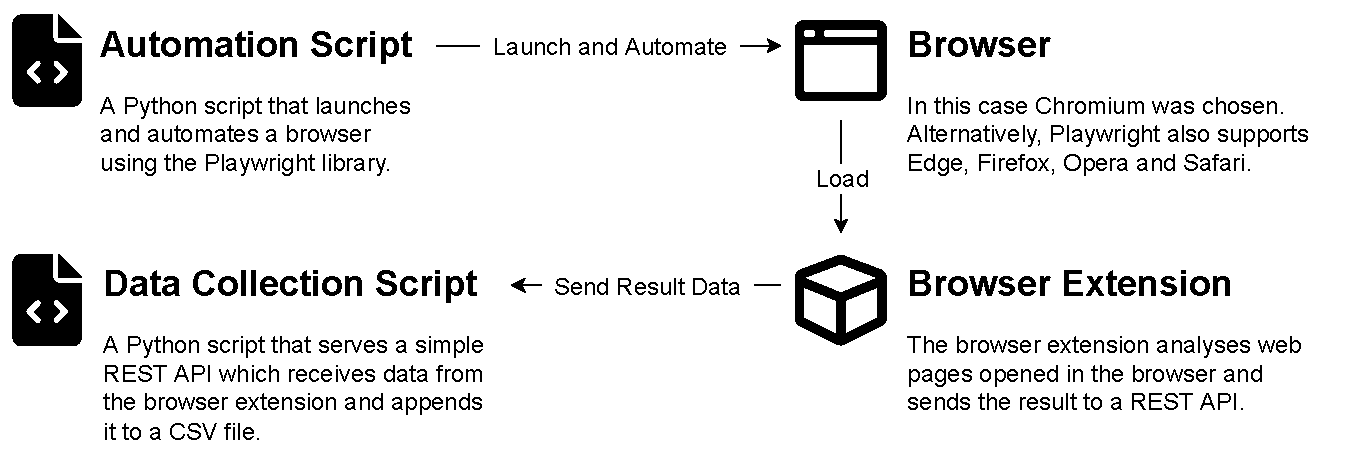
\includegraphics[width=16cm]{img/automation.pdf}
    \caption{Overview of the automation infrastructure}
    \label{fig.automation}
\end{figure}

\filbreak{}

The evaluation presented in this chapter analyzes the \num[round-precision=0]{16000} most popular domains acquired from the Tranco list \cite{Tranco} for the 3rd of May, 2022. The Tranco list was chosen due to its focus on providing a list suitable for research. It has the benefit of being available free of charge and allows reproducible results due to the permanent availability of historical lists. Since the list bases its domain ranking on a combination of data from different datasets such as Alexa, Cisco Umbrella and Majestic, it provides a more accurate representation of real-world popularity and better resistance against manipulation compared to its sources. \cite{Tranco}

Domains are processed in parallel, with limits on how many pages are processed at the same time and how long each page is allowed to load for. After testing different values for these limits, the ideal configuration in terms of performance and reliability for the machine that the automation was tested on seem to be a maximum of twice as much tabs open at the same time as the amount of available \acs{cpu} cores, and a timeout of $75$ to $90$ seconds. The timeouts are necessary in order to prevent pages with long loadings times from accumulating, which would slow down the script and potentially cause it to get stuck waiting indefinitely for unresponsive pages.



\section{Results of the Evaluation}
\label{sec.findings}

This section presents the results of the evaluation of API overwriting in popular websites. The first paragraph discusses the success rate and explains why certain domains included in the Tranco list did not produce a result. The following paragraphs discuss the most commonly overwritten \acsp{api} and present use-cases for these modifications.

Out of the \num[round-precision=0]{16000} domains that where processed, \SI[round-precision=0]{17.91}{\percent} failed to load or did not produce a result. This has various reasons, with the most common one being that not all domains included in the Tranco list host web pages. Domains such as \icode{akamaiedge.net} are used for \acp{cdn}, which act as proxies that cache and deliver resources such as images, audio, videos or scripts. Other domains like \icode{doubleclick.net} serve advertisements, and domains such as \icode{adobe.io} offer \acs{http}~\acsp{api}. Additionally, some domains only redirect to other domains, like \icode{youtu.be} and \icode{bit.ly}. The Tranco list also includes domains that only serve web content on subdomains, but does not include any subdomains (e.g. \icode{sub.example.com}) in the list, only the \ac{esld} (e.g. \icode{example.com}). One example of such a domain is \icode{wixsite.com}, which only serves web content on subdomains in the form of \icode{example.wixsite.com} that can be registered by users.

A visualization of the success rate and the prevalence of certain properties, such as how many sites included external scripts that modified \browserAPIs{}, can be seen in \autoref{fig.evaluation-overview}. The following sections will address these properties in more detail.

\begin{figure}[H]
    \centering
    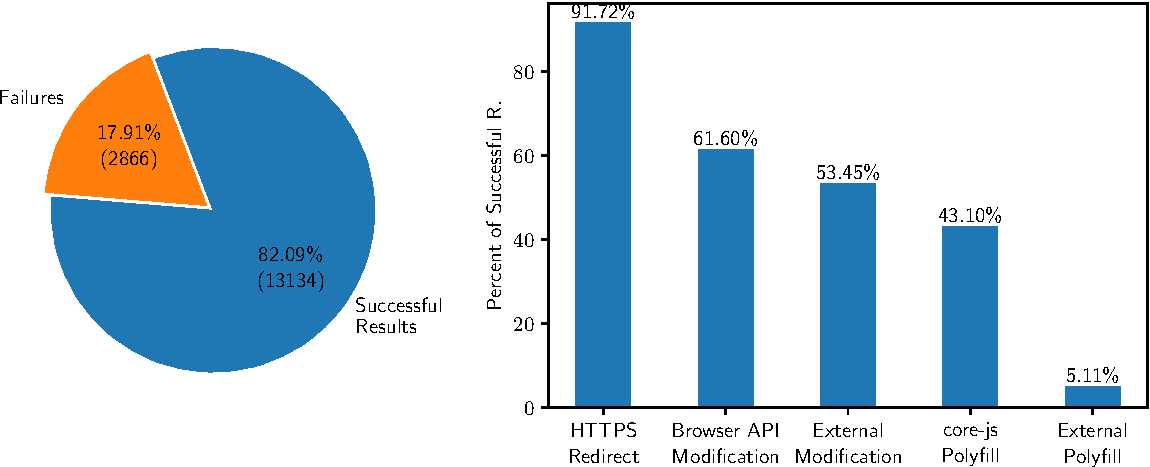
\includegraphics[width=16cm]{img/evaluation-overview.pdf}
    \caption{Failure rate (left) and prevalence of certain properties (right)}
    \label{fig.evaluation-overview}
\end{figure}

The results show that it is common practice to overwrite \acsp{api}, even when an up-to-date browser is used. In total, \SI[round-precision=0]{61.60}{\percent} of the successfully processed domains modified at least one browser \ac{api}. The ten most commonly overwritten \acs{api} methods and the percentage of domains that overwrote them can be seen in \autoref{tab.apisTop10}, while a more extensive list is available in appendix \ref{tab.apis}. With approximately \SI[round-precision=0]{44.12}{\percent} and \SI[round-precision=0]{40.79}{\percent} of affected domains respectively, the two most commonly modified \acsp{api} are \icode{history.pushState()} and \icode{history.replaceState()}. These functions can be used to add items to the browser session history or modify existing items in the history, as long as the URLs of the history items are part of the same origin as the current location \cite{MozPushState, MozReplaceState}. JavaScript libraries such as Google Tag Manager, Meta (formerly known as Facebook) Pixel Tracker and the Tiktok Pixel Tracker overwrite the aforementioned functions to track which pages a user visits and how they interact with the web application. Some domains even include multiple libraries that all overwrite the same function. In the case of \icode{wordpress.com}, the \icode{pushState} function is overwritten by the following five external libraries: Google Tag Manager, Meta Pixel Tracker, Microsoft Clarity (user session recording), Olark (live chat) and Outbrain (advertisement and recommendations). These overwrites each add an additional wrapper around the native browser \acs{api}, but – at least in this case – do not seem to interfere with each other.

\begin{table}[h]
    \parbox{\linewidth}{
    \centering
    \begin{tabular}{|r|l|}
    \hline
    Percentage & API Method \\
    \hline
    44.12 & \minline{history.pushState}\\
    40.79 & \minline{history.replaceState}\\
    13.64 & \minline{fetch}\\
    11.88 & \minline{setTimeout}\\
     8.22 & \minline{setInterval}\\
     6.96 & \minline{Math.sinh}\\
     6.76 & \minline{parseInt}\\
     6.79 & \minline{requestAnimationFrame}\\
     6.62 & \minline{clearTimeout}\\
     6.57 & \minline{XMLHttpRequest}\\
    \hline
    \end{tabular}
    }
    \caption{Top 10 most commonly modified APIs and percentage of affected domains}
    \label{tab.apisTop10}
\end{table}

\filbreak{}

The results also make it clear that the usage of polyfill libraries is very common. The polyfill library core-js is used by \SI[round-precision=0]{43.10}{\percent} of domains and more than \SI[round-precision=0]{5.11}{\percent} of web applications included polyfills from third-party domains. \autoref{tab.polyfill-domains} shows the 10 most popular services for external polyfills, with the most common one being \icode{polyfill.io}.

The low amount of externally included polyfill libraries seems to indicate that the libraries are usually hosted on first-party domains or subdomains, which is a good way to reduce the attack surface since there is less trust being placed on third-parties. It is surprising, however, to see government pages such as \icode{www.texas.gov} and even financial platforms such as \icode{www.blockchain.com} include external scripts from third-parties such as \icode{polyfill.io}.

\begin{table}[h]
    \centering
    \begin{tabular}{|r|l|}
    \hline
    Percent & Domain \\
    \hline
    2.84 & polyfill.io\\
    0.30 & gannettdigital.com\\
    0.29 & cloudflare.com\\
    0.24 & alicdn.com\\
    0.13 & jsdelivr.net\\
    0.13 & cloudfront.net\\
    0.12 & jwpcdn.com\\
    0.09 & squarespace.com\\
    0.06 & unpkg.com\\
    0.06 & wp.com\\
    \hline
    \end{tabular}
    \caption{Top 10 most common third-party domains delivering polyfill libraries and percentage of successfully analyzed domains using them}
    \label{tab.polyfill-domains}
\end{table}

The list of modified functions only includes a single instace where an existing cryptography \acsp{api} was overwritten, which will be investigated in \autoref{sec.investigationOfObfuscatedFunc}. In this case, however, there was no evidence for the threats as described in \autoref{sec.threats.crypto}. There are two cases in which websites added new functions to the crypto \acs{api}. These new functions are not used as replacements for existing functionality, but instead offer utilities for converting between different encodings (such as bytes, hexadecimal or base64) and an implementation of the cryptographically insecure md5 hash algorithm.

A browser \acs{api} that is commonly overwritten, is the fetch \acs{api}. With \SI[round-precision=0]{13.64}{\percent} of the analyzed domains modifying \icode{fetch}, it is the third most commonly overwritten browser \acs{api}. Investigations of some of these cases has revealed that this is done to customize its behavior and monitor web applications. This is also done by the “sentry” library for example, which overwrites \icode{fetch} and \icode{console} methods to monitor and collect data about the behavior of web applications. As listed in \autoref{tab.modifying-domains}, sentry modifies browser \acsp{api} in \SI[round-precision=2]{0.49}{\percent} of the scanned domains.

Since the automation script opens \acp{url} with the insecure \acs{http} by default, it was also measured how many web servers automatically redirect to \acs{https}, as instructed by the browser via the \icode{Upgrade-Insecure-Requests} header which all browsers are required to send along with insecure requests \cite{UpgradeInsecureRequests}. Out of the successfully processed domains, \SI[round-precision=0]{91.72}{\percent} redirected to \acs{https}. The domains that do not redirect to \acs{https} include government websites such as \icode{www.chinatax.gov.cn}, which also does not use a trusted certificate authority and therefore browsers show a security warning when manually specifying that \acs{https} should be used.

\section{Case Study of an Obfuscated API Overwrite}
\label{sec.investigationOfObfuscatedFunc}

This section will investigate an overwrite of the \icode{crypto.getRandomValues()} \ac{api} by an obfuscated script. The overwrite was detected during the automated evaluation and identified on the real estate web application \icode{zillow.com}.

The function that \icode{crypto.getRandomValues()} was replaced with is depicted in \autoref{lst.obfuscatedFunc}. Due to the obfuscation technique, it is not apparent how this function behaves. Furthermore, the code references variables such as \icode{c} and \icode{t} that are defined outside of the function.

\begin{lstlisting}[language=JavaScript,breaklines=true,breakatwhitespace=false,label={lst.obfuscatedFunc},caption={Obfuscated function}]
function n(){try{var i=3===++c,o=this&&Object.getPrototypeOf(this)===n.prototype||!1,u={P:o?null:this,L:Array.prototype.slice.call(arguments),$:null},a=!1;if(i)lu(Error(),E);else if(r)try{r(u)}catch(t){a=!0}if(o?u.P=u.$=Le(t,$e(u.L)):u.$=t.apply(u.P,u.L),!i&&!a&&e)try{e(u)}catch(t){}return u.$}finally{c--}}
\end{lstlisting}

In order to attempt to reverse engineer the function, the script responsible for the overwrite was examined. The URL of the script is \icode{https://www.zillow.com/HYx10rg3/init.js}, which means that it does not originate from a third-party domain. However, it is possible that this code was included by a third-party JavaScript library. This seems to be the case, as the file contains a header with the following comment:\\
\icode{// @license Copyright (C) 2014-2022 PerimeterX, Inc (www.perimeterx.com).}\\
\icode{Content of this file can not be copied and/or distributed.} % haha, we will see about that lol

The relevant content of the file is listed in \autoref{lst.obfuscatedScript}. Line breaks and indentation were added to improve the readablility. While the code is still difficult to understand, we can see that the function \icode{n} from \autoref{lst.obfuscatedFunc} is contained in the lines 5 to 32 of \autoref{lst.obfuscatedScript}. Some of the previously unknown variables are defined in lines 2 to 4 and received as arguments in line 1. The function in line 33 to 48 creates properties on the object \icode{t} and overwrites its \icode{toString()} method, which suggests that \icode{t} is the \browserAPI{} being overwritten and this is an attempt at hiding the true string value, which would reveal that the \ac{api} was overwritten.

\begin{lstlisting}[language=JavaScript,breaklines=true,breakatwhitespace=true,label={lst.obfuscatedScript},caption={Content of obfuscated script}]
function qe(t, n) {
    var r = n._ || null
        , e = n.U || null
        , c = 0
        , i = function n() {
        try {
            var i = 3 === ++c
                , o = this && Object.getPrototypeOf(this) === n.prototype || !1
                , u = {
                P: o ? null : this,
                L: Array.prototype.slice.call(arguments),
                $: null
            }
                , a = !1;
            if (i)
                lu(Error(), E);
            else if (r)
                try {
                    r(u)
                } catch (t) {
                    a = !0
                }
            if (o ? u.P = u.$ = Le(t, $e(u.L)) : u.$ = t.apply(u.P, u.L),
            !i && !a && e)
                try {
                    e(u)
                } catch (t) {}
            return u.$
        } finally {
            c--
        }
    };
    return function(t, n) {
        try {
            Object.defineProperty(t, "name", {
                value: n.name
            })
        } catch (t) {}
        try {
            Object.defineProperty(t, "length", {
                value: n.length
            })
        } catch (t) {}
        "function" == typeof n.toString && (t.toString = function() {
            return n.toString()
        }
        )
    }(i, t),
    i
}
\end{lstlisting}

Using the additional context gained through the surrounding code, an attempt was made to reverse engineer the function \icode{n} in line 5 of \autoref{lst.obfuscatedFunc}. First, a break-point was set at the beginning of the function through the Chromium developer tools. Next, the function was called with \icode{crypto.getRandomValues(new Uint32Array(42));} and then stepped through, in order to assess its behavior. During each step, the values of the variables were noted down to get a better understanding of their use. The final reverse engineered function is shown in \autoref{lst.reverseEngineeredFunc}. Variables have been renamed to reflect their purpose and the code has been restructured in order to improve readability.

While some functions and variables referenced in the code of \autoref{lst.reverseEngineeredFunc} are still not entirely s, the function previously called \icode{n} seems to be designed to act as a wrapper around the native \ac{api}. The wrapper function allows adding hooks that are called before and after the native \ac{api}. In this case, \icode{preHook} references another function and \icode{postHook} is undefined. The \icode{preHook} function, which is defined in another section of the code that is not included here, checks if the requested type for the random values is \icode{Uint8Array} and has the length \icode{16}. Calling \icode{rypto.getRandomValues(new Uint8Array(16));} results in the hook executing further functions, however, those do not manipulate the returned value.

\filbreak{}

Since the wrapper function calls the native \icode{crypto.getRandomValues()} API and returns its result unmodified, this does not seem to be a malicious \browserAPI{} overwrite. However, the complete behavior of the function could not be reverse engineered due to the high complexity and obfuscation of the code.

While this case study could not identify malicious behavior, it demonstrates the complexity involved in reverse engineering and classifying whether manipulations are malicious.

\par{}

\begin{lstlisting}[language=JavaScript,breaklines=true,breakatwhitespace=false,label={lst.reverseEngineeredFunc},caption={Attempt at reverse engineering the obfuscated function}]
/* Variables defined outside */
// Reference to original function
var nativeGetRandomValues = crypto.getRandomValues;

var preHook = wrapper.preHook || null
var postHook = wrapper.postHook || null

// Counter of failed attempts
var attempts = 0;

/* The function "n" */
function wrapperFunc() {
    try {
        // Increase attempts, check if this is the third (unsuccessfull) attempt
        var isThirdAttempt = 3 === ++attempts;
        // this === Crypto
        var calledOnSelf = this && Object.getPrototypeOf(this) === wrapper.prototype || false;
        // calledOnSelf = false
        var obj = {
            // thisOrNull === Crypto
            thisOrNull: calledOnSelf ? null : this,
            // Copy arguments into args
            args: Array.prototype.slice.call(arguments),
            result: null
        }
        var preHookFailed = false;

        if (isThirdAttempt) {
            // Log stack trace?
            funcA(Error(), E);
            // E === 13 (error code?)
        } else if (preHook) {
            try {
                preHook(obj);
            } catch (error) {
                preHookFailed = true;
            }
        }

        if (calledOnSelf) {
            obj.result = Le(nativeGetRandomValues, funcB(u.args))
            obj.thisOrNull = u.result
        } else {
            // Call original function
            obj.result = nativeGetRandomValues.apply(obj.thisOrNull, obj.args);
        }

        // If all contitions are true:
        // 1) result has a value
        // 2) it is not the third (failed) attempt
        // 3) preHook did not fail
        // 4) postHook is defined
        if (obj.result, !isThirdAttempt && !preHookFailed && postHook) {
            // Try calling postHook
            try {
                postHook(obj)
            } catch (error) {
                /* ignore errors */
            }
        }

        // Return result
        return obj.result
    } finally {
        // decrease (failed) attempts
        attempts--
    }
}
\end{lstlisting}



% ============================= Mitigations ============================
\chapter{Mitigation and Best Practices}
\label{sec.mitigation}

This chapter provides recommendations that reduce the attack surface and improve security in order to mitigate the attacks presented in \autoref{sec.threats} and address issues uncovered in the evaluation results in \autoref{sec.findings}. The recommendations are divided into sections that address specific roles and responsibilities: \autoref{sec.mitigation.webdev} focuses on best practices for web developers, \autoref{sec.mitigation.webserver} provides recommendations for administrators on how to properly configure web servers and monitor web applications. Finally, \autoref{sec.mitigation.user} explains what users can do to protect themselves.

\section{Best Practices for Web Developers}
\label{sec.mitigation.webdev}

Whenever possible, web developers should avoid including JavaScript libraries from external domains that are not guaranteed to be trustworthy to reduce the attack surface. Depending on the web application and target audience it might be necessary to include scripts from \acp{cdn} or service providers such as Google. If the content of included scripts is not expected to change, as is generally the case for content hosted on \acp{cdn}, web developers can configure security policies that prevent the execution of these scripts if their content was manipulated. This can be done by generating \ac{sri} hashes of the script files and adding those hashes to the \icode{integrity} attribute of the script elements. When the configured hash does not match the hash of the script, the browser will refuse to execute the code and show an error in the developer console. \cite{MozSRI}

Furthermore, developers should minimize the amount of dependencies of their applications and carefully analyze libraries from third-parties to reduce the possibility of including malicious code. If polyfills are required, it should be ensured that polyfills only overwrite native browser \acp{api} when necessary. To verify the behavior of web applications and the libraries that they include, developers can use browser extensions such as the one implemented in \autoref{sec.browserExtension}.

\section{Web Server Configuration and Application Monitoring}
\label{sec.mitigation.webserver}

To ensure a secure connection and prevent manipulation through \ac{mitm} attacks, web servers need to support \acs{https} and use valid certificates. As specified by the W3C, servers should honor the \icode{Upgrade-Insecure-Requests} header sent by browsers and redirect to a secure \acs{url} \cite{UpgradeInsecureRequests}. It is also important to configure secure settings for the \ac{tls} protocol. Mozilla provides a simple configuration generator that supports various server software including common web servers such as Apache and Nginx, which can be found here: \url{https://ssl-config.mozilla.org/}.

\filbreak{}

Furthermore, administrators should regularly perform automated scans of their web applications in order to make sure that scripts are only included from trusted domains and behave as expected. This could be done using the automation infrastructure described in \autoref{sec.automation-architecture}.

Web servers should also configure security policies such as the \acs{csp} explained in \autoref{sec.csp} to limit the origins of where resources are allowed to be included from. The \acs{csp} also allows administrators to monitor the inclusion of disallowed resources through reports generated and sent by browsers that support the policy.



\section{Advice for Users}
\label{sec.mitigation.user}

While users can use the browser extension implemented in \autoref{sec.browserExtension} to become aware of potentially harmful browser API overrides, deciding whether overrides are actually malicious unfortunately requires technical knowledge about the specific web application. It is, however, possible for users to reduce the likelyhood of manipulation by preventing the execution of JavaScript from domains that are known to be malicious.

Browser extensions such as uBlock Origin can be used to block advertisements, trackers and scripts from malicious domains. Advertisement services not only pose a risk to the users privacy by collecting information, but also increase the attack surface when advertisements are not properly sandboxed and able to execute code that could override browser \acsp{api} of the page they are included in. As discovered through the evaluation in \autoref{sec.findings}, trackers commonly overwrite browser \acsp{api}, which can pose a security risk. As an alternative to uBlock, more advanced users can use extensions such as uMatrix to create granular filter rules based on the origin of included resources that can be configured to block the execution of third-party scripts unless explicitly allowed.



% ============================= Conclusion =============================
\chapter{Conclusion and Outlook}
\label{sec.conclusion}

This thesis set out to assess the threats that browser \ac{api} overwriting poses and investigate the prevalence of browser \ac{api} overwriting on real-world websites. In order to determine the prevalence, a browser extension and an automated analysis tool were developed and used to conduct an empirical evaluation of the \num[round-precision=0]{16000} most popular websites of the Tranco list.

While \ac{api} overwriting requires an attacker to be able to execute JavaScript code in a web application, the related work and threat model presented here show that there are circumstances in which this is possible. The assessment of the potential threats posed by browser \ac{api} overwriting revealed that such overwriting can be used by an attacker to compromise the integrity and confidentiality of data from users of the affected web application. Depending on the web application, it is also possible to compromise the security of passwords and cryptographic keys generated by web applications.

The evaluation determined that it is common practice to overwrite \acsp{api}, even when an up-to-date browser is used. In total, \SI[round-precision=0]{61.60}{\percent} of the successfully processed domains modified at least one browser \ac{api}. The results also show that more than half (\SI[round-precision=0]{53.45}{\percent}) of the sites include external scripts that modify browser APIs. The most common use for \ac{api} overwriting is the tracking of user interactions for analytics purposes.

The thesis presented possible approaches to mitigate the threats of \ac{api} manipulation and made recommendations for web developers, administrators and users that reduce the attack surface in order to prevent malicious \ac{api} manipulation. The recommendations focus on preventing the execution of code from unknown sources and reducing the amount of external dependencies.

The browser extension developed as part of this thesis can be used by web developers to verify the behavior of their web applications. In addition, the automated analysis tool can be modified in order to continually analyze specific sites of a web application to ensure that it overwrites \acsp{api} only when intended and only from sources that are trusted.

Further research is needed to create automated systems that are able to reliably classify whether detected \ac{api} modifications are malicious or legitimate. It might be possible to apply similar approaches as used by antivirus software to generate and compare signatures against known malicious JavaScript code. As this might be defeated by code obfuscation, it would also be possible to make use of function hooking to trace the behavior of unknown code and classify it using heuristic algorithms.



% ============================= Appendices =============================
\begin{appendices}


%\chapter{Evaluation Results}

\begin{landscape}
    \label{sec.appendix}

    % Increase chapter counter
    \stepcounter{chapter}

    \begin{table}
    
    % Add entry to TOC
    \addcontentsline{toc}{chapter}{\protect\numberline{\thechapter}Evaluation Results}
    \label{sec.appendix-evaluation}

    \RawFloats
    \parbox{.45\linewidth}{
        \centering
        \begin{tabular}{|r|l|}
        \hline
        Percentage & API Method \\
        \hline
        44.12 & \minline{history.pushState}\\
        40.79 & \minline{history.replaceState}\\
        13.64 & \minline{fetch}\\
        11.88 & \minline{setTimeout}\\
         8.22 & \minline{setInterval}\\
         6.96 & \minline{Math.sinh}\\
         6.76 & \minline{parseInt}\\
         6.79 & \minline{requestAnimationFrame}\\
         6.62 & \minline{clearTimeout}\\
         6.57 & \minline{XMLHttpRequest}\\

         6.43 & \minline{console.error}\\
         6.39 & \minline{parseFloat}\\
         5.70 & \minline{webkitRequestAnimationFrame}\\
         4.90 & \minline{queueMicrotask}\\
         4.68 & \minline{Promise}\\
         4.06 & \minline{MutationObserver}\\
         3.67 & \minline{getComputedStyle}\\
         3.56 & \minline{console.log}\\
         3.52 & \minline{console.warn}\\
         3.37 & \minline{console.info}\\
         2.84 & \minline{Request}\\
         2.84 & \minline{console.debug}\\
         2.49 & \minline{alert}\\
         2.16 & \minline{confirm}\\
         2.12 & \minline{clearInterval}\\
        \hline
        \end{tabular}
        \caption{Top 25 most commonly modified APIs and percentage of affected domains}
        \label{tab.apis}
    }
    \hfill{}
    \parbox{.45\linewidth}{
        \centering
        \begin{tabular}{|r|l|}
        \hline
        Percentage & Domain \\
        \hline
        24.23 & googletagmanager.com\\
        19.06 & facebook.net\\
         4.90 & clarity.ms\\
         4.34 & cloudflareinsights.com\\
         2.57 & tiktok.com\\
         2.56 & adobedtm.com\\
         1.40 & outbrain.com\\
         0.94 & driftt.com\\
         0.92 & tinypass.com\\
         0.91 & hsleadflows.net\\
         0.65 & cloudflare.com\\
         0.63 & perfectmarket.com\\
         0.59 & hsforms.net\\
         0.57 & visualwebsiteoptimizer.com\\
         0.57 & hscollectedforms.net\\
         0.53 & vimeo.com\\
         0.52 & go-mpulse.net\\
         0.52 & sentry-cdn.com\\
         0.50 & yektanet.com\\
         0.48 & quantummetric.com\\
         0.48 & heapanalytics.com\\
         0.47 & alicdn.com\\
         0.46 & datadoghq-browser-agent.com\\
         0.46 & realsrv.com\\
         0.42 & foresee.com\\
        \hline
        \end{tabular}
        \caption{Top 25 most common domains of scripts which modify browser APIs}
        \label{tab.modifying-domains}
    }

    \end{table}

\end{landscape}

\chapter{Source Code and Licenses}

The source code of the software developed as part of this thesis can be found here:

\begin{itemize}
	\item \url{https://github.com/irgendwr/wam-detector} (browser extension and automation scripts)
	\item \url{https://github.com/irgendwr/bachelor-thesis} (source code of this document)
	\item On the DVD included in the physical copy of this document
\end{itemize}

The code is licensed under the MIT license. A copy of the license is distributed alongside it.

The text of this thesis, its \LaTeX{} source code and figures that do not include icons by Font Awesome (i.e.~\ref{fig.scope}, \ref{fig.browser-process-model}, \ref{fig.evaluation-overview}) are licensed under the \href{http://creativecommons.org/licenses/by/4.0/}{Creative Commons Attribution 4.0 International (CC BY 4.0) license}.

Figures that include icons by Font Awesome (i.e.~\ref{fig.threat-model-components}, \ref{fig.browser-extension-context}, \ref{fig.automation}) are subject to the terms and conditions of the \href{https://fontawesome.com/license}{Font Awesome license} and licensed under the \href{http://creativecommons.org/licenses/by-nd/4.0/}{Creative Commons Attribution-NoDerivatives 4.0 International (CC BY-ND 4.0) license}, provided that it does not conflict with the terms and conditions of the \href{https://fontawesome.com/license}{Font Awesome license}.

\end{appendices}



% ================================ Lists ===============================
\begingroup
    \footnotesize
    \listoffigures
    \addcontentsline{toc}{chapter}{List of Figures, Tables and Listings}
    \let\clearpage\relax
    \listoftables
    \lstlistoflistings
\endgroup


% ============================== Acronyms ==============================
\chapter*{Acronyms}
\addcontentsline{toc}{chapter}{Acronyms}

\begin{acronym}[HTTPS ]\itemsep4pt
    \acro{api}[API]{Application Programming Interface}
    \acroplural{api}[APIs]{Application Programming Interfaces}
    \acro{css}[CSS]{Cascading Style Sheets}
    \acro{cdn}[CDN]{Content Delivery Network}
    \acroplural{cdn}[CDNs]{Content Delivery Networks}
    \acro{cpu}[CPU]{Central Processing Unit}
    \acro{csp}[CSP]{Content Security Policy}
    \acro{csv}[CSV]{Comma-Separated Values}
    \acro{dom}[DOM]{Document Object Model}
    \acro{ddos}[DDoS]{distributed denial-of-service}
    \acro{dos}[DoS]{denial-of-service}
    \acro{esld}[eSLD]{effective second-level domain}
    \acroplural{esld}[eSLDs]{effective second-level domains}
    \acro{etld}[eTLD]{effective top-level domain}
    \acroplural{etld}[eTLDs]{effective top-level domains}
    \acro{gpu}[GPU]{Graphics Processing Unit}
    \acro{html}[HTML]{Hypertext Markup Language}
    \acro{http}[HTTP]{Hypertext Transfer Protocol}
    \acro{https}[HTTPS]{Hypertext Transfer Protocol Secure}
    \acro{ipc}[IPC]{inter-process communication}
    \acro{isp}[ISP]{Internet service provider}
    \acroplural{isp}[ISPs]{Internet service providers}
    \acro{json}[JSON]{JavaScript Object Notification}
    \acro{mitm}[MITM]{man-in-the-middle}
    \acro{os}[OS]{operating system}
    \acroplural{os}[OSs]{operating systems}
    \acro{prng}[PRNG]{pseudo-random number generator}
    \acroplural{prng}[PRNGs]{pseudo-random number generators}
    \acro{psl}[PSL]{Public Suffix List}
    \acro{rest}[REST]{Representational State Transfer}
    \acro{sld}[SLD]{second-level domain}
    \acroplural{sld}[SLDs]{second-level domains}
    \acro{sri}[SRI]{Subresource Integrity}
    \acro{ssl}[SSL]{Secure Sockets Layer}
    \acro{tcp}[TCP]{Transmission Control Protocol}
    \acro{tld}[TLD]{top-level domain}
    \acroplural{tld}[TLDs]{top-level domains}
    \acro{tls}[TLS]{Transport Layer Security}
    \acro{udp}[UDP]{User Datagram Protocol}
    \acro{ui}[UI]{user interface}
    \acro{uri}[URI]{Uniform Resource Identifier}
    \acroplural{uri}[URIs]{Uniform Resource Locators}
    \acro{url}[URL]{Uniform Resource Locator}
    \acroplural{url}[URLs]{Uniform Resource Locators}
    \acro{xss}[XSS]{Cross-Site Scripting}
\end{acronym}



% ============================= References =============================
% see references.bib

% add all entries in the bib file to the bibliography
\nocite{*}

% print references
\begin{raggedright}
	\printbibliography[title=References]
\end{raggedright}



% ====================== Eidesstattliche Erklärung =====================
\chapter*{Eidesstattliche Erklärung}

Hiermit versichere ich an Eides statt, dass ich die vorliegende Arbeit im Bachelorstudiengang Software-System-Entwicklung selbstständig verfasst und keine anderen als die angegebenen Hilfsmittel – insbesondere keine im Quellenverzeichnis nicht benannten Internet-Quellen – benutzt habe. Alle Stellen, die wörtlich oder sinngemäß aus Veröffentlichungen entnommen wurden, sind als solche kenntlich gemacht. Ich versichere weiterhin, dass ich die Arbeit vorher nicht in einem anderen Prüfungsverfahren eingereicht habe und die eingereichte schriftliche Fassung der elektronischen Abgabe entspricht.

Ich stimme der Einstellung der Arbeit in die Bibliothek des Fachbereichs Informatik zu.

\vspace{1cm}

\begin{tabular}{ll}
    \centering
    \makebox[5cm]{\hrulefill} & \makebox[8cm]{\hrulefill}\\
    Ort, Datum & Unterschrift \\
\end{tabular}



% ============================== Todo List =============================
\listoftodos
% \todototoc

\end{document}
